% La parte central del trabajo refiere a lo que es producción propia o aporte del
% proyecto de grado, incluyendo las decisiones tomadas. Por ejemplo, puede incluir
% los requerimientos, el análisis y el diseño de la solución. Si el proyecto tiene una
% implementación, debe describirse en términos de decisiones tomadas en ese sentido.
% Los detalles de programación se dejan para los anexos.

% Se pueden incluir figuras en el documento, las mismas deben estar referenciadas en el texto. Por ejemplo, la Figura~\ref{fig:logos} muestra los logos de Facultad de Ingeniería y de la Universidad de la República.

% \begin{figure}[h!]
%     \centering
%     
\includegraphics[width=\textwidth]{figs/logo-udelar-fing.png}
%     \caption{Logos de FIng y UdelaR}
%     \label{fig:logos}
% \end{figure}

\graphicspath{{chapters/3_diseño/figures/}}

% parte central
\chapter{Voxel cone tracing}\label{chap:design}

En este capítulo se detalla el diseño de \textit{voxel cone tracing} \cite{voxel-cone-tracing}, un algoritmo de iluminación global en tiempo real, que utiliza conceptos presentes en el trazado de rayos (\ref{sec:ray-tracing}) y \textit{photon mapping} (\ref{sec:photon-mapping}).
Reduce los costos asociados a estos algoritmos clásicos trazando conos en lugar de rayos (\ref{sec:historical-cone-tracing}) y usando una representación de la escena de vóxeles (\ref{sec:voxels}) almacenada en un \textit{octree} disperso (\ref{sec:octree}).

Otra forma de reducir costos y aumentar la velocidad del algoritmo es reutilizar el ducto raster \ref{sec:graphics-pipeline} y renderizado diferido \ref{sec:deferred-rendering}.
Los cálculos de luz se realizan en el \textit{fragment shader} del ducto de raster, sobre los \textit{geometry buffers} para reducir la cantidad de fragmentos o hilos de la gpu sobre los que se corren calculos pesados, sin perder calidad de imagen.
Esto difiere del trazado de rayos clásico, que renderiza toda la escena puramente mediante intersecciones entre rayos y geometría.

% TODO: Este párrafo es nuevo, así que hay que darle una pasada
La principal aproximación que realiza el algoritmo es trabajar sobre una representación voxelizada pre-filtrada de la escena.
Se recorre el árbol usando las coordenadas para hallar un vóxel que represente esa región del espacio.
Este vóxel contiene toda la información necesaria sobre oclusión, color, irradiancia, debido a que la estructura es previamente filtrada.
En el filtrado, la información parte de las hojas del árbol y es promediada hacia niveles mayores hasta que todo el árbol tiene información.
La información del vóxel en ese nivel resume la información de todos los hijos.
Se vió en la sección sobre trazado de conos, que en su planteo original, se hallaban las intersecciones del cono con los objetos de la escena de manera analítica, lo que es costoso.
Aquí, en lugar de hallar la intersección analiticamente, se muestrean distintos puntos a lo largo del cono.
En cada punto, se toma el diámetro del cono y se usa para calcular el nivel del \textit{octree} necesario, dado que nivels mas altos del octree son una aproximación de sus hijos con menos lujo de detalle.
Esto permite acumular la información a lo largo del cono de manera rápida.

% Estaría bueno poner diagramas de cada etapa:
% - Voxelización: no se qué hacer
% - Construcción y filtrado
% - Inyección de fotones: puedo poner un dibujo de rayos saliendo de la fuente de luz
% - Trazado de conos: poner un cono agarrando varios vóxeles

El algoritmo se puede dividir en 4 grandes etapas:

\begin{enumerate}
    \item Voxelización de la escena
    \item Construcción y filtrado del \textit{octree} disperso
    \item Inyección de fotones
    \item Trazado de conos
\end{enumerate}

La voxelización, la inyección de fotones y el trazado de conos usan el ducto raster, mientras que la construcción del árbol y el filtrado usan el ducto de cómputo de propósito general.
En el resto del capítulo se explicará con mayor grado de detalle cada una de estas etapas.

\section{Voxelización}\label{sec:voxelization}

La escena se divide en una grilla de vóxeles.
La cantidad de vóxeles es configurable, siendo usualmente $512$ o $1024$ por dimensión.

Para voxelizar la escena, se realiza el procedimiento detallado en ``OpenGL Insights, capítulo 22'' \cite{opengl-insights}, un aporte escrito por Crassin luego de haber publicado el artículo de \textit{voxel cone tracing}, aprovechando mejoras en las herramientas disponibles en el momento.
Ese mismo proceso será explicado a continuación, para más información, consultar la referencia.

Usando la rendering pipeline de OpenGL, se procesan todos los triángulos de la geometría de la escena.
Esto genera una lista de \textbf{vóxeles}, en los que se almacena la posición y el color del triángulo original.
Cada uno de estos vóxeles será usado para construir el árbol y terminará almacenado en la estructura.

La voxelización de un triángulo $B$ a un vóxel $V$ puede hacerse si:

\begin{enumerate}
    \item El plano de $B$ interseca $V$.
    \item La proyección 2D del triángulo $B$ por la dimensión dominante de su normal (la que provee la mayor área proyectada) interseca la proyección 2D de $V$.
\end{enumerate}

Basado en esta observación, se sigue la serie de pasos que se muestra en la figura \ref{fig:voxelization_pipeline}.

\begin{figure}[h!]
    \centering
    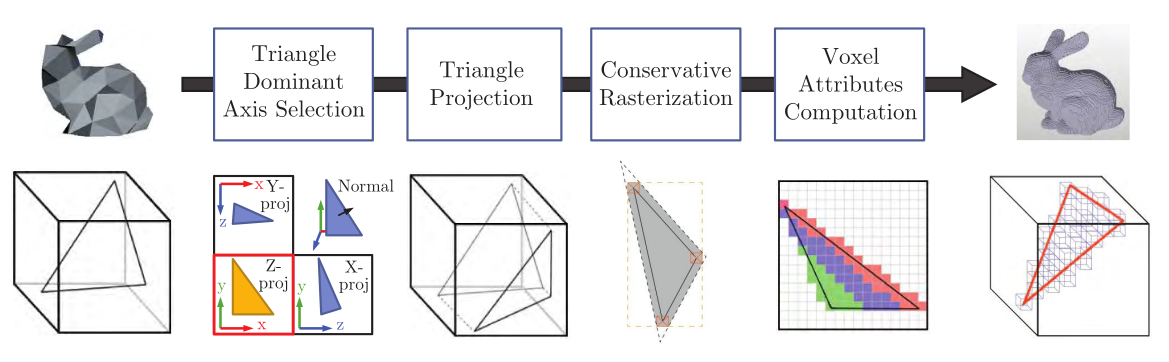
\includegraphics[width=\textwidth]{voxelization_pipeline.png}
    \caption{Ducto de voxelización. Fuente: \cite{opengl-insights}}
    \label{fig:voxelization_pipeline}
\end{figure}

Primero, cada triángulo de la geometría se proyecta ortográficamente en la dimensión dominante de su normal.
La dimensión dominante se elige dinámicamente por triángulo en el \textit{geometry shader}, donde la información de los tres vértices de cada triángulo está disponible.
Esto se realiza para maximizar el area del triangulo proyectado.

Cada triángulo proyectado se rasteriza para conseguir fragmentos correspondientes a la resolución 3D de la grilla de vóxeles.
Se fija el tamaño del \textit{viewport} a coincidir con la cantidad de vóxeles, por ejemplo un \textit{viewport} de tamaño $512\times512$ para una grilla de $512^3$ vóxeles.
% Mientras se hace esto, se mantienen las operaciones del framebuffer desactivadas, como el depth testing. % TODO: Habría que explicar por qué, no entendí del capítulo de OpenGL Insights

Durante la rasterización, cada triángulo genera un conjunto de fragmentos 2D.
Debido a la elección de la dimensión dominante de la normal para la proyección, solo pueden intersecar con 3 vóxeles en profundidad. % TODO: Por qué? No se explicarlo sin algun dibujo :sweat-smile:
Entonces, por cada fragmento 2D, los vóxeles que intersecaron con el triángulo se calculan en el \textit{fragment shader}, basándose en la posición, la profundidad y las derivadas en espacio de pantalla. % TODO: Hacemos lo de las derivadas?

Luego de realizada la voxelización, se obtiene la lista de vóxeles necesaria para crear el árbol, con su posicion, color y normal.
Estos vóxeles son una generalización en 3D de los fragmentos 2D.
Cada uno tiene una coordenada que lo identifica dentro de la grilla 3D de la escena, así como color y posición.

\subsection{Rasterización conservativa}

El método descrito anteriormente a veces no crea vóxeles para elementos muy finos, como un asta de bandera.
Esto pasa porque en el rasteriado del ducto raster solo se prueba el centro del píxel contra los triángulos para generar fragmentos. % TODO: Revisar en el código
Se necesita una manera de generar fragmentos para cada píxel tocado por un triángulo, no necesariamente en el centro.
Un algoritmo así se detalla en \cite{conservative-rasterization}.

La idea es generar, por cada triángulo, un polígono acotante ligeramente más grande, para asegurarse que cualquier triángulo proyectado que toca un pixel (en cualquier punto) también toca su centro.
Esto se hace alargando las aristas del triángulo hacia afuera, la mitad de la diagonal de un pixel, generando un triangulo semejante.
Hay fragmentos que resultan de sobreestimar la cobertura de este triángulo, dado que este nuevo triangulo puede tocar el centro de pixeles que antes no tocaba.
Para evitar este problema tambien se genera una caja acotante alineada con los ejes, y se descartan fragmentos por fuera de la misma.
Este proceso se muestra en la figura \ref{fig:conservative_rasterization}.

% TODO: Cambiar por una foto nuestra?
\begin{figure}[h!]
    \centering
    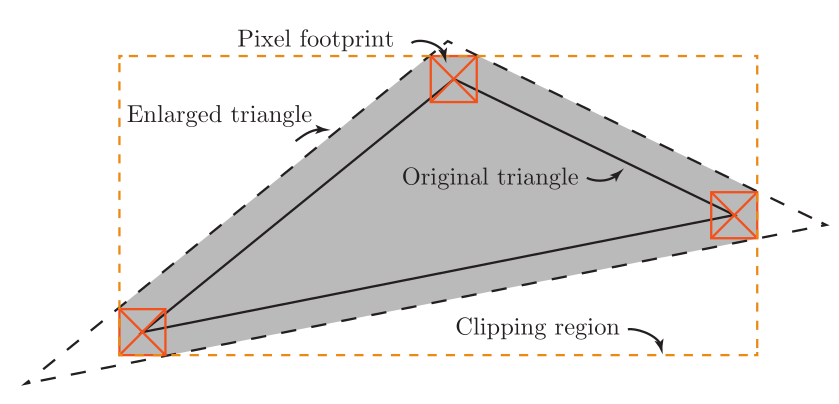
\includegraphics[width=\textwidth]{conservative_rasterization.png}
    \caption{Rasterización conservativa. Fuente: \cite{opengl-insights}}
    \label{fig:conservative_rasterization}
\end{figure}

\section{\textit{Octree} disperso}

Para almacenar los vóxeles generados, se usa un \textit{octree} disperso, como los vistos en la sección \ref{sec:octree}.
Esta estructura subdivide la escena en $8$ y cada hijo en $8$ y así sucesivamente.
Al ser disperso, puede ser que ciertos hijos no se subdividan si no hay más geometría dentro de la región de la escena que representan.

Cada elemento del árbol es un \textbf{nodo}.
Un nodo del árbol representa una sección de la escena.
Cada nivel tiene una cierta cantidad de nodos.
Si el árbol fuera denso, cada nivel $n$ tendría $8^n$ nodos.
El nivel $0$ tendría $1$ nodo, el nivel $1$ tendría $8$, el $2$ $64$ y así sucesivamente.
Al ser un árbol disperso, no se crean nodos para regiones de la escena que no contienen geometría.
El último nivel del árbol es el que llega a la resolución deseada de $512$ o $1024$ vóxeles.
Valores más altos de resolución crean más niveles del \textit{octree} y hacen que se asemeje cada vez más la aproximación de vóxeles a la geometría real.

% TODO: Podría agregar fotos de la visualización del octree a distintas resoluciones

Dado que la estructura tiene como máximo $512$ o $1024$ vóxeles de resolución, sin importar la geometría de la escena, los cálculos sobre ella son independientes de la complejidad de la geometría.

\subsection{Nodos y bricks}\label{sec:nodes_and_bricks}

Los nodos del árbol no almacenan los vóxeles mencionados en \ref{sec:voxelization}.
Cada nodo almacena únicamente un puntero a sus, como máximo $8$, hijos.

Cada nodo tiene asociado un \textbf{brick}, otra estructura que también representa una región del espacio.
Cada brick está dividido en 27, $3\times3\times3$, vóxeles.
Son estos vóxeles los que almacenan los valores de la escena.
En la figura \ref{fig:node_and_brick} se puede observar un nodo con su brick asociado de la manera en la que se disponen en el espacio.
Los bricks ocupan más espacio que sus nodos, esto es porque los vóxeles se centran en sus vértices.
Esto es útil para que los bricks puedan obtener valores de sus vecinos, lo que garantiza que la interpolación dentro de un solo brick toma en cuenta los valores de sus vecinos.
Esto resulta en una frontera compartida entre vecinos, como se puede ver en la figura \ref{fig:brick_border_overlap}.
Esta frontera debe almacenar lo mismo para que la interpolación a la hora de generar la imagen final funcione.
Un \textit{shader} llamado \textit{border\_transfer}, es el que se encarga de lograr la coherencia en la frontera entre dos \textit{bricks}.
Se explicará en la sección \ref{sec:border_transfer}.

\begin{figure}[h!]
    \centering
    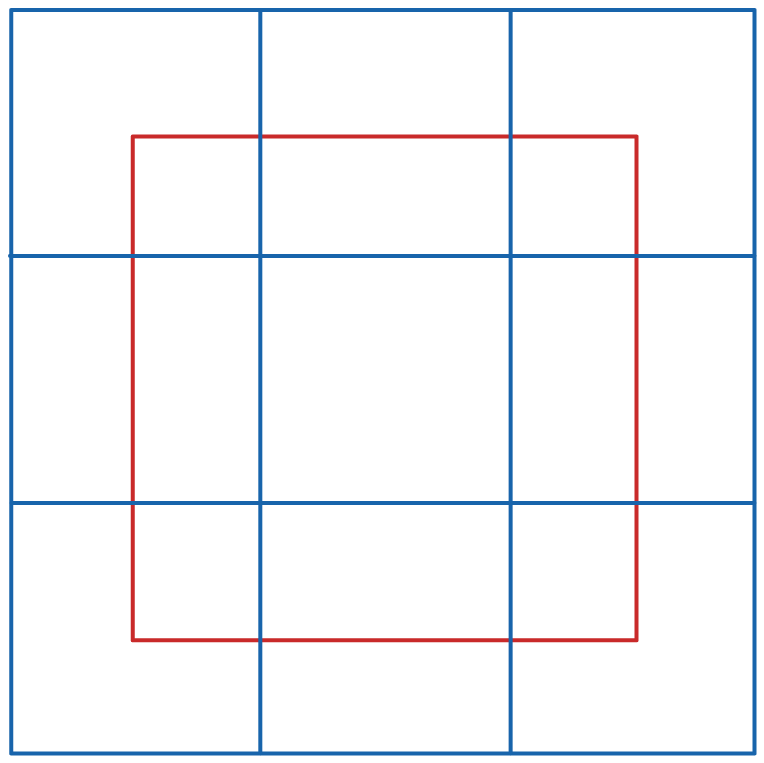
\includegraphics[width=.3\textwidth]{node-and-brick.png}
    \caption{Nodo (en rojo) con su brick asociado (azul)}
    \label{fig:node_and_brick}
\end{figure}

\begin{figure}[h!]
    \centering
    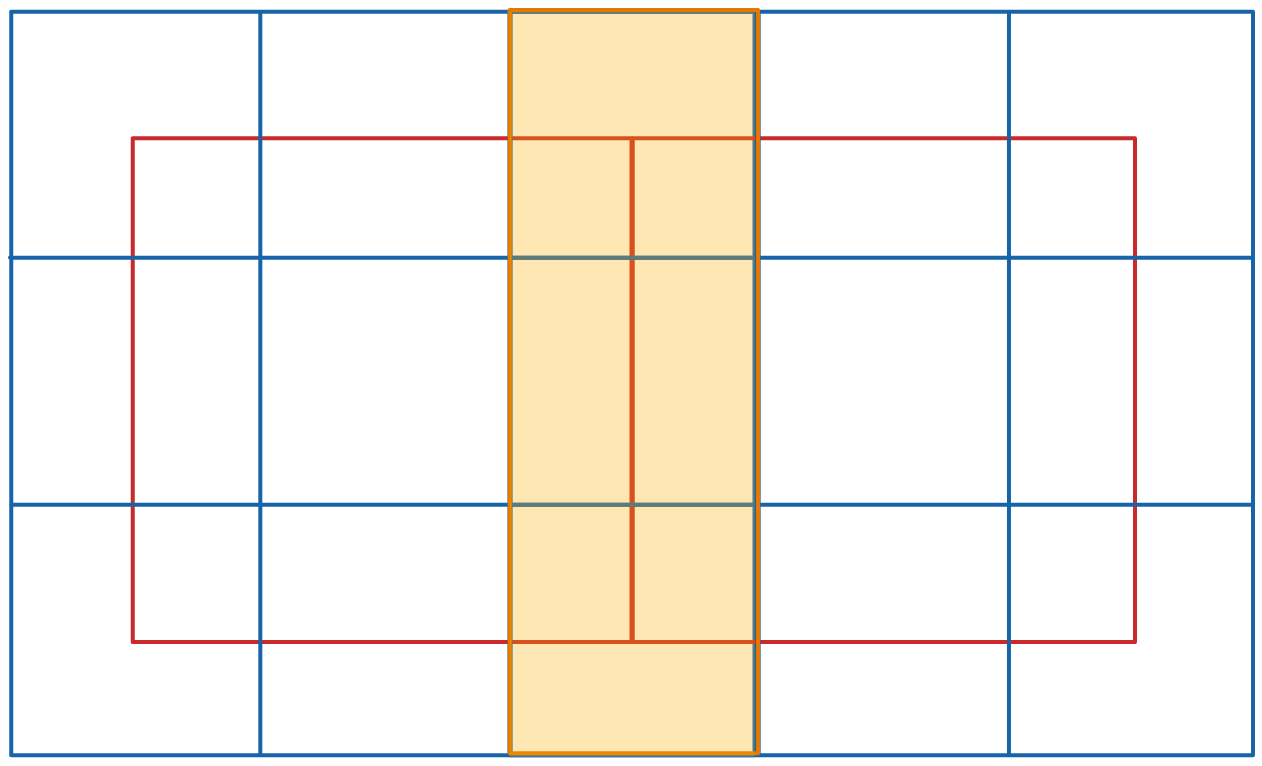
\includegraphics[width=.5\textwidth]{brick-border-overlap.png}
    \caption{Solapamiento entre vóxels de bricks de nodos vecinos}
    \label{fig:brick_border_overlap}
\end{figure}

\subsection{Construcción}\label{design:svo_construction}

Para generar esta estructura se usa la lista de vóxeles generada durante la voxelización.
Se empieza con un árbol con un solo nivel, con un solo nodo que ocupa toda la escena.
Se ejecuta el algoritmo a continuación sobre este nivel para generar el siguiente, y luego se continúa aplicándolo en cada nivel del árbol hasta completarlo.

% TODO: Dibujos para explicar flag y allocate

Dado un nivel $i$ del árbol, dos programas principales son ejecutados en secuencia para generar el nivel $i + 1$: \textit{flag\_nodes} y \textit{allocate\_nodes}.

Se corre un hilo de \textit{flag\_nodes} por cada vóxel de la lista de vóxeles.
Dado un vóxel, se recorre el árbol construido hasta el momento, hasta que se llega a una sección del nodo no subdividida.
Esta sección del nodo se marca para ser subdividida.

Luego, se ejecuta \textit{allocate\_nodes}, que busca en el nivel $i$ secciones marcadas para subdividir.
Al encontrar una sección de un nodo marcada, crea un nuevo nodo en la estructura y cambia la marca por un puntero a ese nuevo nodo.

Siempre y cuando haya un fragmento en la región de la escena representada por un nodo, este será subdividido nivel tras nivel.

Una vez alcanzado el último nivel, se escriben los atributos de los vóxeles en los bricks de las hojas del árbol, promediando cuando más de uno tiene la misma posición en la grilla de vóxeles.
Esto último pasa más mientras más triángulos tiene la escena original y menos resolución tiene la grilla de vóxels.
Las hojas no tienen hijos.

En \ref{sec:nodes_and_bricks}, se vió como los bricks ocupan una región más amplia del espacio.
% TODO: Habría que explicar que los vóxeles son un octavo de nodo del último nivel. Para que esto tenga sentido.
Para consolidar esto con el tamaño de los vóxels, estos se almacenan únicamente en las esquinas de los bricks.
Se almacenan en la esquina más cercana a la posición del vóxel.
Luego, se aplica un programa \textit{spread\_leaves}, para esparcir estos valores a lo largo de todo el brick.
Esto funciona de la siguiente manera, la cual se muestra en 2D en la figura \ref{fig:spread-leaves}:
\begin{itemize}
    \item El vóxel central almacena el promedio de todas las 8 esquinas
    \item El vóxel del medio de cada cara almacena el promedio de las 4 esquinas de su cara
    \item El vóxel del medio de cada arista almacena el promedio de las 2 esquinas de esa arista
\end{itemize}
De esta manera, se esparcen los valores de las esquinas a todo el brick.
Este es el algoritmo que expande los vóxeles generados poder llenar los bricks $3\times3\times3$.
A partir de aquí, el termino ``vóxel'' refiere a una de las $27$ subdivisiones de un brick, dado que ya se procesó la lista generada durante la voxelización.

\begin{figure}
    \begin{subfigure}{.5\textwidth}
        \centering
        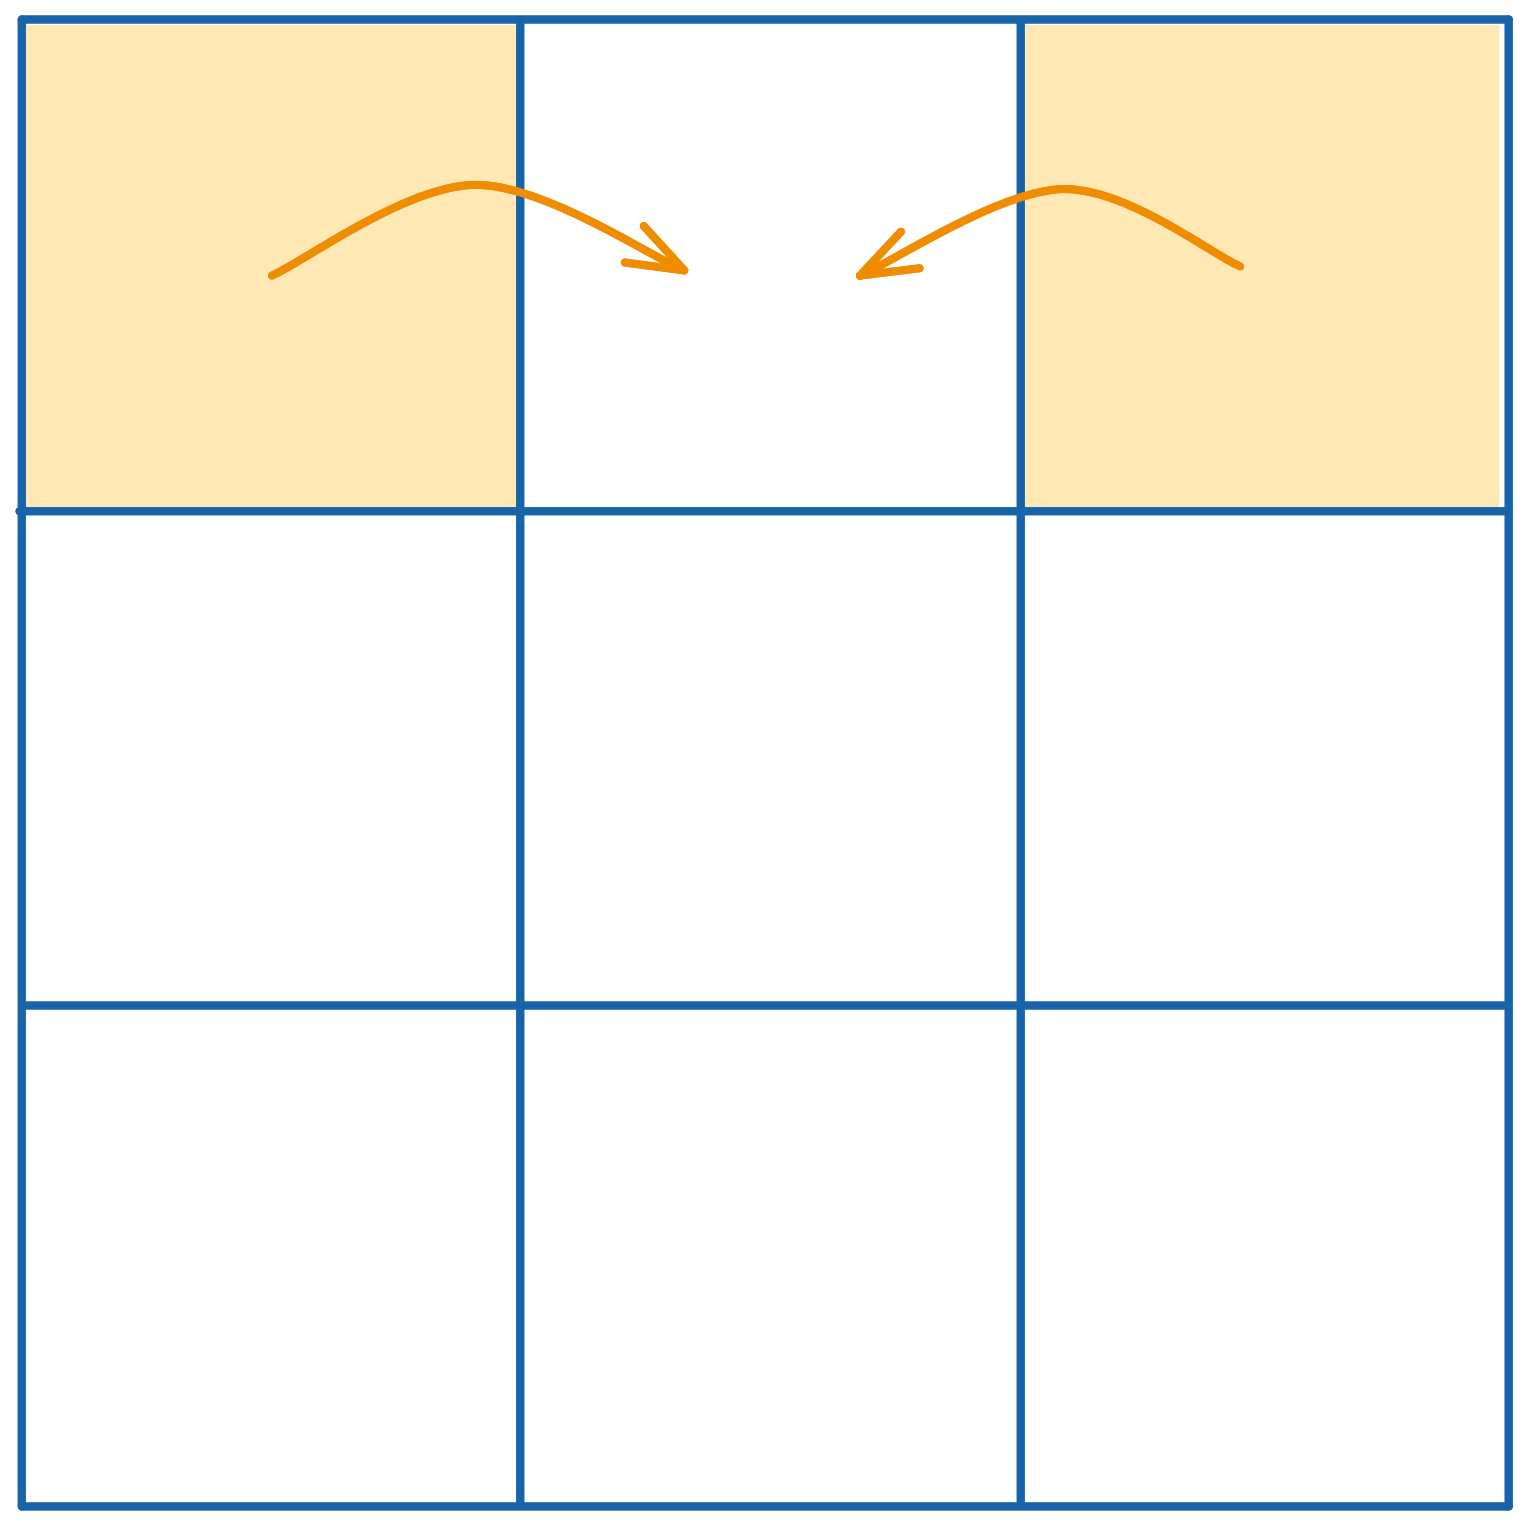
\includegraphics[width=.75\textwidth]{spread-leaves-edge.png}
        \caption{En una arista}
    \end{subfigure}
    \begin{subfigure}{.5\textwidth}
        \centering
        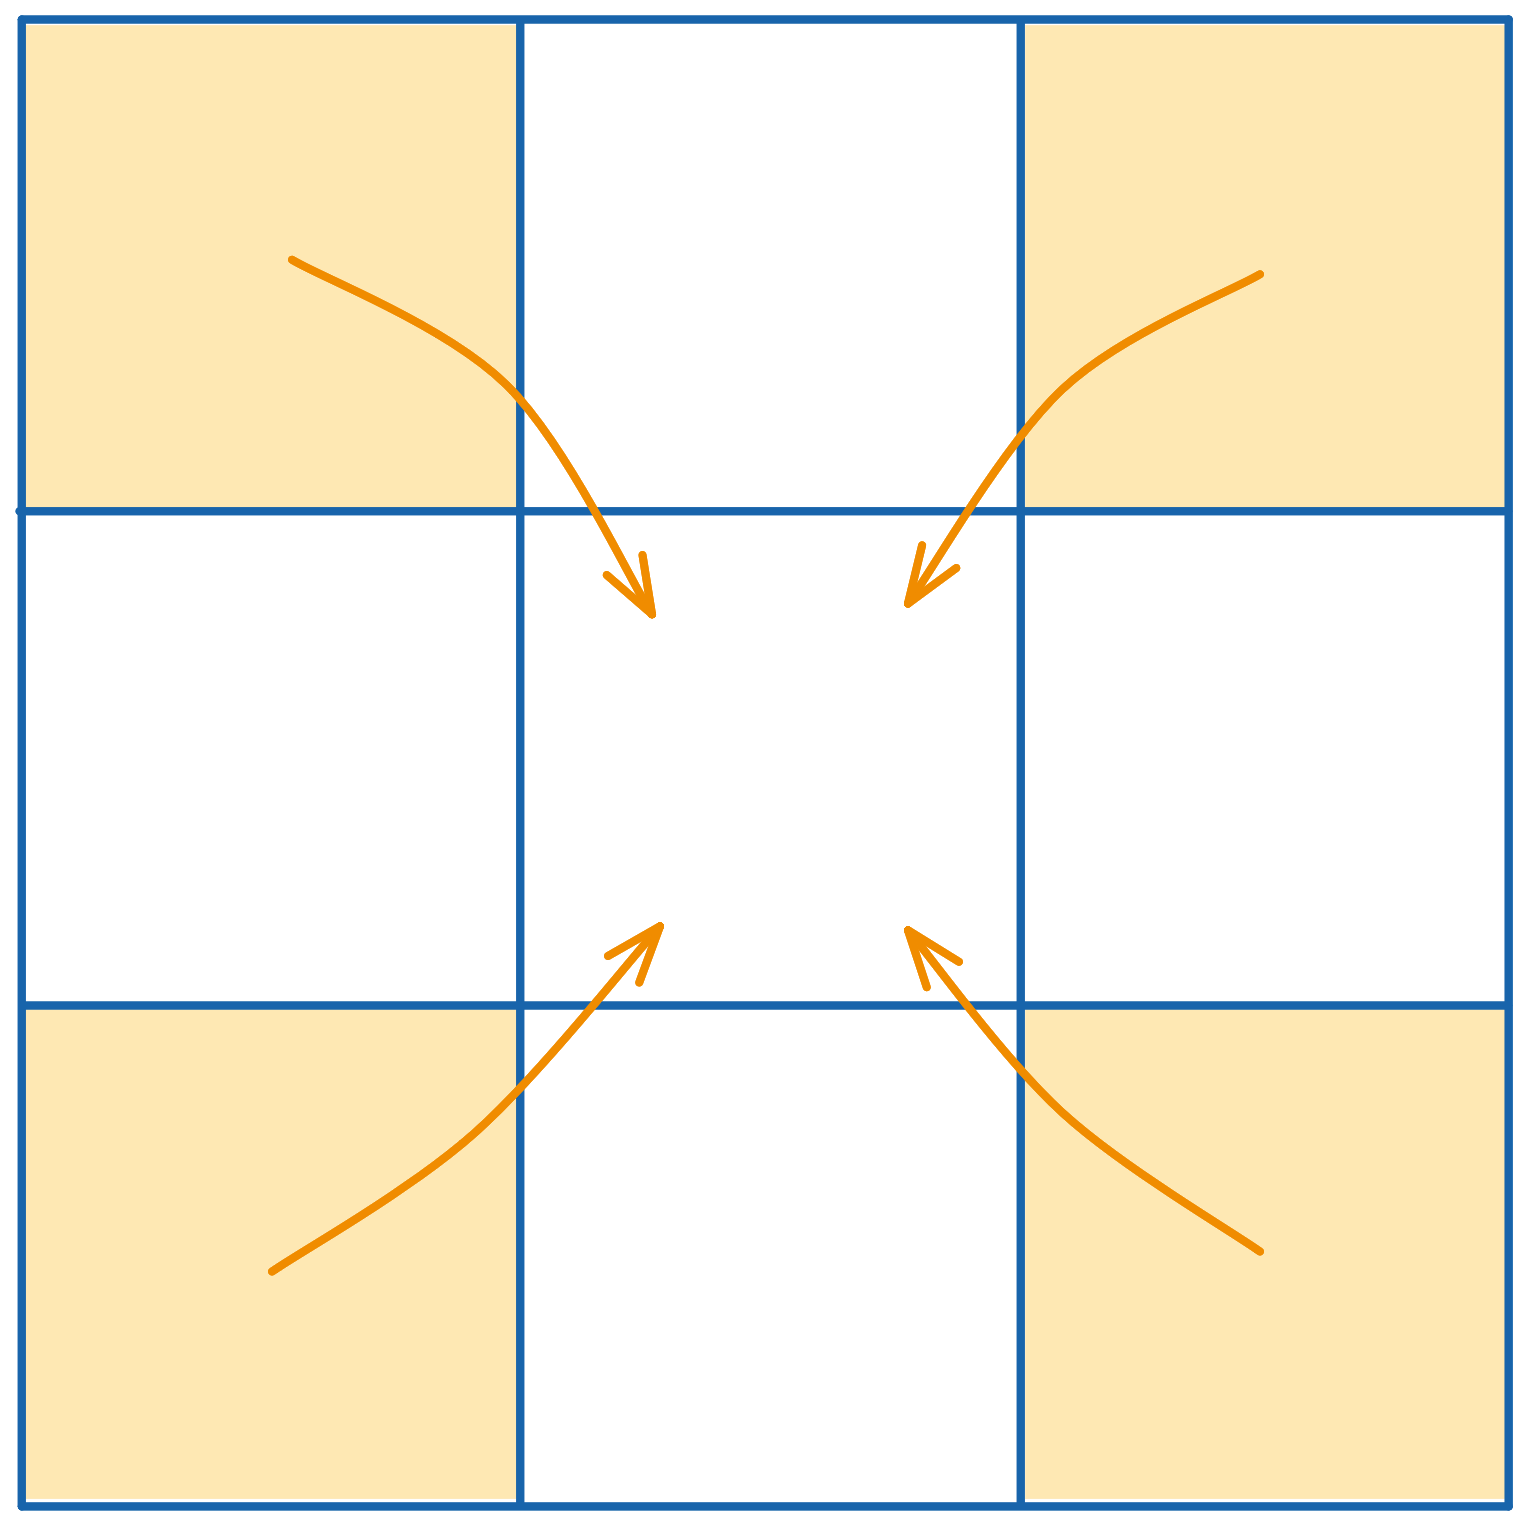
\includegraphics[width=.75\textwidth]{spread-leaves-center.png}
        \caption{En el centro}
    \end{subfigure}
    \caption{Funcionamiento de \textit{spread\_leaves} en 2D. Las flechas indican aporte al promedio}
    \label{fig:spread-leaves}
\end{figure}

\subsection{Border transfer}\label{sec:border_transfer}

Como se mencionó anteriormente, las fronteras entre bricks son compartidas, corresponden al mismo espacio en la escena.
Por lo tanto, los valores almacenados en esos vóxeles deben ser los mismos.
Esto garantiza una correcta interpolación a la hora de generar la imagen final.
Sin embargo, luego de \textit{spread\_leaves}, esta frontera tiene valores distintas en cada brick vecino.
Para igualarlos, se promedian los valores de la frontera con la del brick vecino, asegurandose que el nivel sea coherente.
De esto se encarga \textit{border\_transfer}.
Este programa promedia los valores en la frontera de cada brick con la de sus vecinos, en X, Y y Z.
De esta manera, aún cuando un vóxel puede estar en varios bricks, en $8$ como máximo, su valor va a ser siempre el mismo en cada uno de ellos.

% TODO: Dibujos para explicar border transfer

\subsection{Nodos frontera}

Al usar un octree disperso, no existen nodos donde no hay geometría.
Esto tiene un problema.
El border transfer asume que todos nodo tiene un vecino, pero esto se rompe cuando se consideran los nodos que tienen como vecinos espacio vacio. Esto rompe nuestro modelo ya que la ausencia de un nodo simboliza espacio vacio, pero los bricks de los nodos tiene datos que son compartidos con otros nodos. Entonces un nodo vecino de espacio vacio puede tener que el voxel que comparte con el espacio vacio es rojo, mientras que la ausencia de nodo en el espacio vacio marca que ese mismo voxel es transparente.
Para que la interpolación continue y logre difuminar el sombreado, es preciso una capa de nodos extra, los que llamaremos \textbf{nodos frontera}, entre la geometría y el espacio vacío.
Estos nodos se añaden en cada nivel del árbol a la hora de construírlo.
Sus bricks no contienen valores, existen solo para interpolar los valores con 0 y difuminar los bordes de la geometría. De esta forma los voxels compartidos por espacio vacio y geometria tienen un promedio de ambas, similar al resto de los voxeles compartidos entre nodos.
El mismo problema no se genera entre estos nuevos nodos y el espacio vacio, dado que los voxels compartidos con el espacio vacio van a tener como valor total transparencia, por lo que terminamos con una estructura consistente.
% TODO: Dibujos para explicar nodos frontera

\subsection{Filtrado}\label{design:filtering}

Una vez que todos los atributos se encuentran en las hojas del octree, estos deben ser filtrados a posiciones superiores.
Filtrarlos implica promediarlos de tal manera que para un nodo interior (no hoja) $A$, su brick tenga un promedio de la información contenida en los bricks de todos sus hijos.
Esto se realiza en $n - 1$ pasos, con $n$ el máximo nivel del octree.
En cada paso, se calcula el valor de cada vóxel del brick del padre, usando los bricks de los hijos.

Consideremos un nodo en el penúltimo nivel, con su brick asociado y sus hijos, como muestra la figura \ref{fig:node_with_children}.
En este caso se muestran solo $4$ hijos porque es en 2D, en lugar de $8$ como en el caso tridimensional.
Cada hijo tiene a su vez su propio brick asociado como se muestra en la figura \ref{fig:all_child_bricks}.

\begin{figure}[h!]
    \centering
    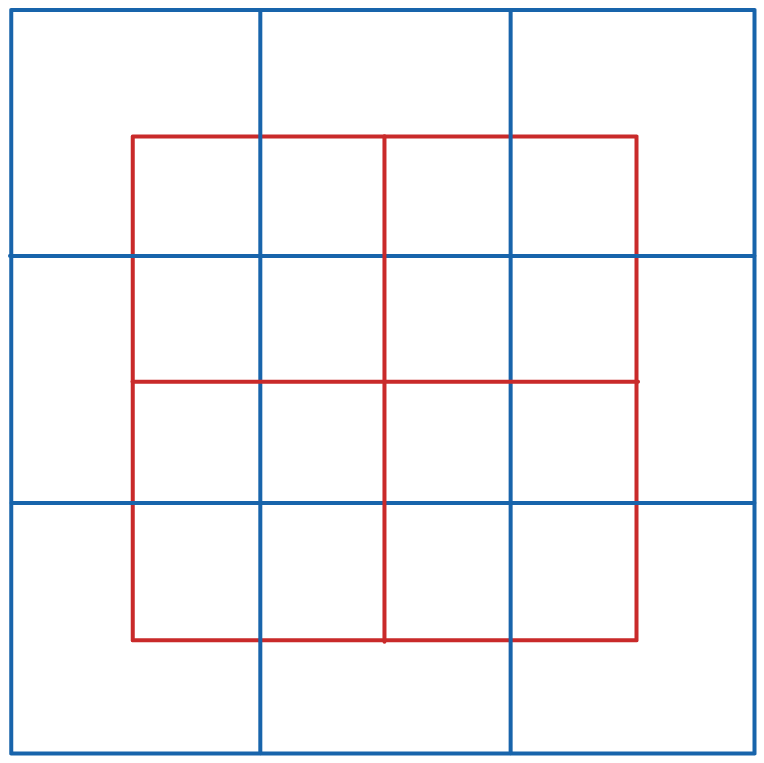
\includegraphics[width=.3\textwidth]{node-with-children.png}
    \caption{Nodo con su brick asociado y sus hijos}
    \label{fig:node_with_children}
\end{figure}

\begin{figure}[h!]
    \begin{center}
        \begin{subfigure}{.24\textwidth}
            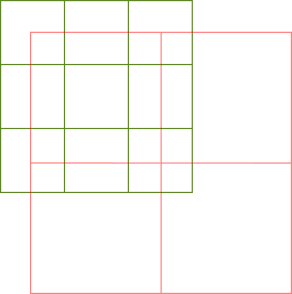
\includegraphics[width=\textwidth]{first-child-brick.png}
        \end{subfigure}
        \begin{subfigure}{.24\textwidth}
            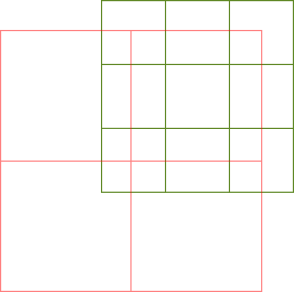
\includegraphics[width=\textwidth]{second-child-brick.png}
        \end{subfigure}
        \begin{subfigure}{.24\textwidth}
            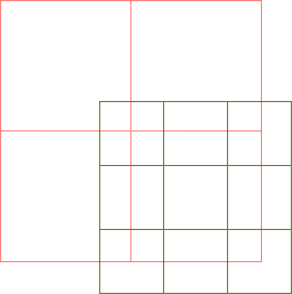
\includegraphics[width=\textwidth]{third-child-brick.png}
        \end{subfigure}
        \begin{subfigure}{.24\textwidth}
            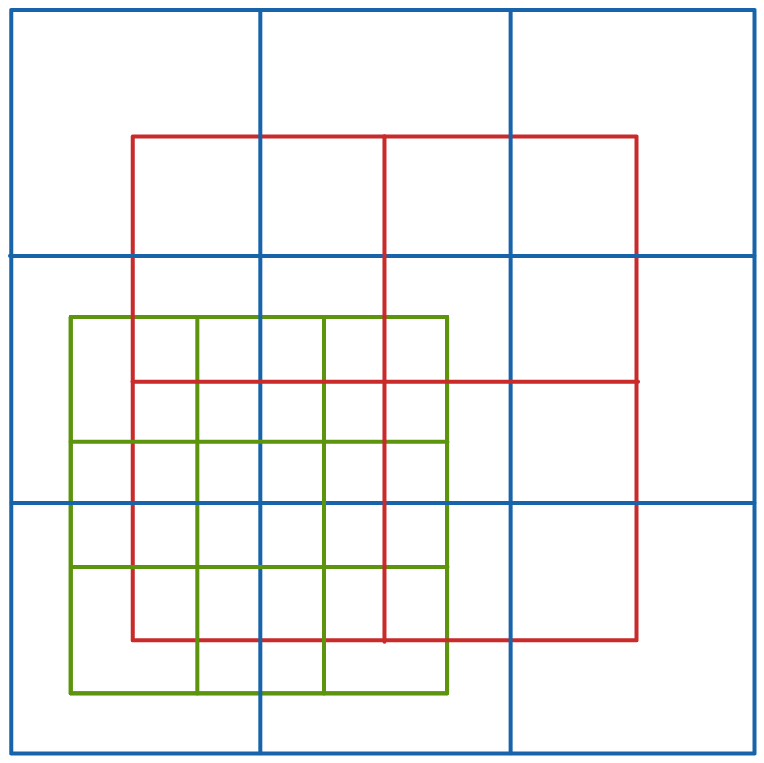
\includegraphics[width=\textwidth]{fourth-child-brick.png}
        \end{subfigure}
    \end{center}
    \caption{Bricks de todos los hijos del nodo}
    \label{fig:all_child_bricks}
\end{figure}

Los valores de los vóxeles del brick padre se calculan en 4 etapas distintas, dependiendo de dónde se ubican en el \textit{brick}: Esquinas, bordes, caras, centro.
Cada una de estas etapas calcula un valor parcial para un tipo de vóxel.
Es parcial porque para los vóxeles limítrofes con otro nodo, este valor tiene que luego ser agregado con el de los vecinos, con un tipo de \textit{border\_transfer}.

% El cálculo para cada etapa es el mismo para todos los vóxeles dentro de su grupo, por lo que se mostrará únicamente el calculo para un vóxel de cada grupo: esquinas, bordes, caras, y centro.
% En el caso 2D, no existe el vóxel centro.

\begin{figure}
    \centering
    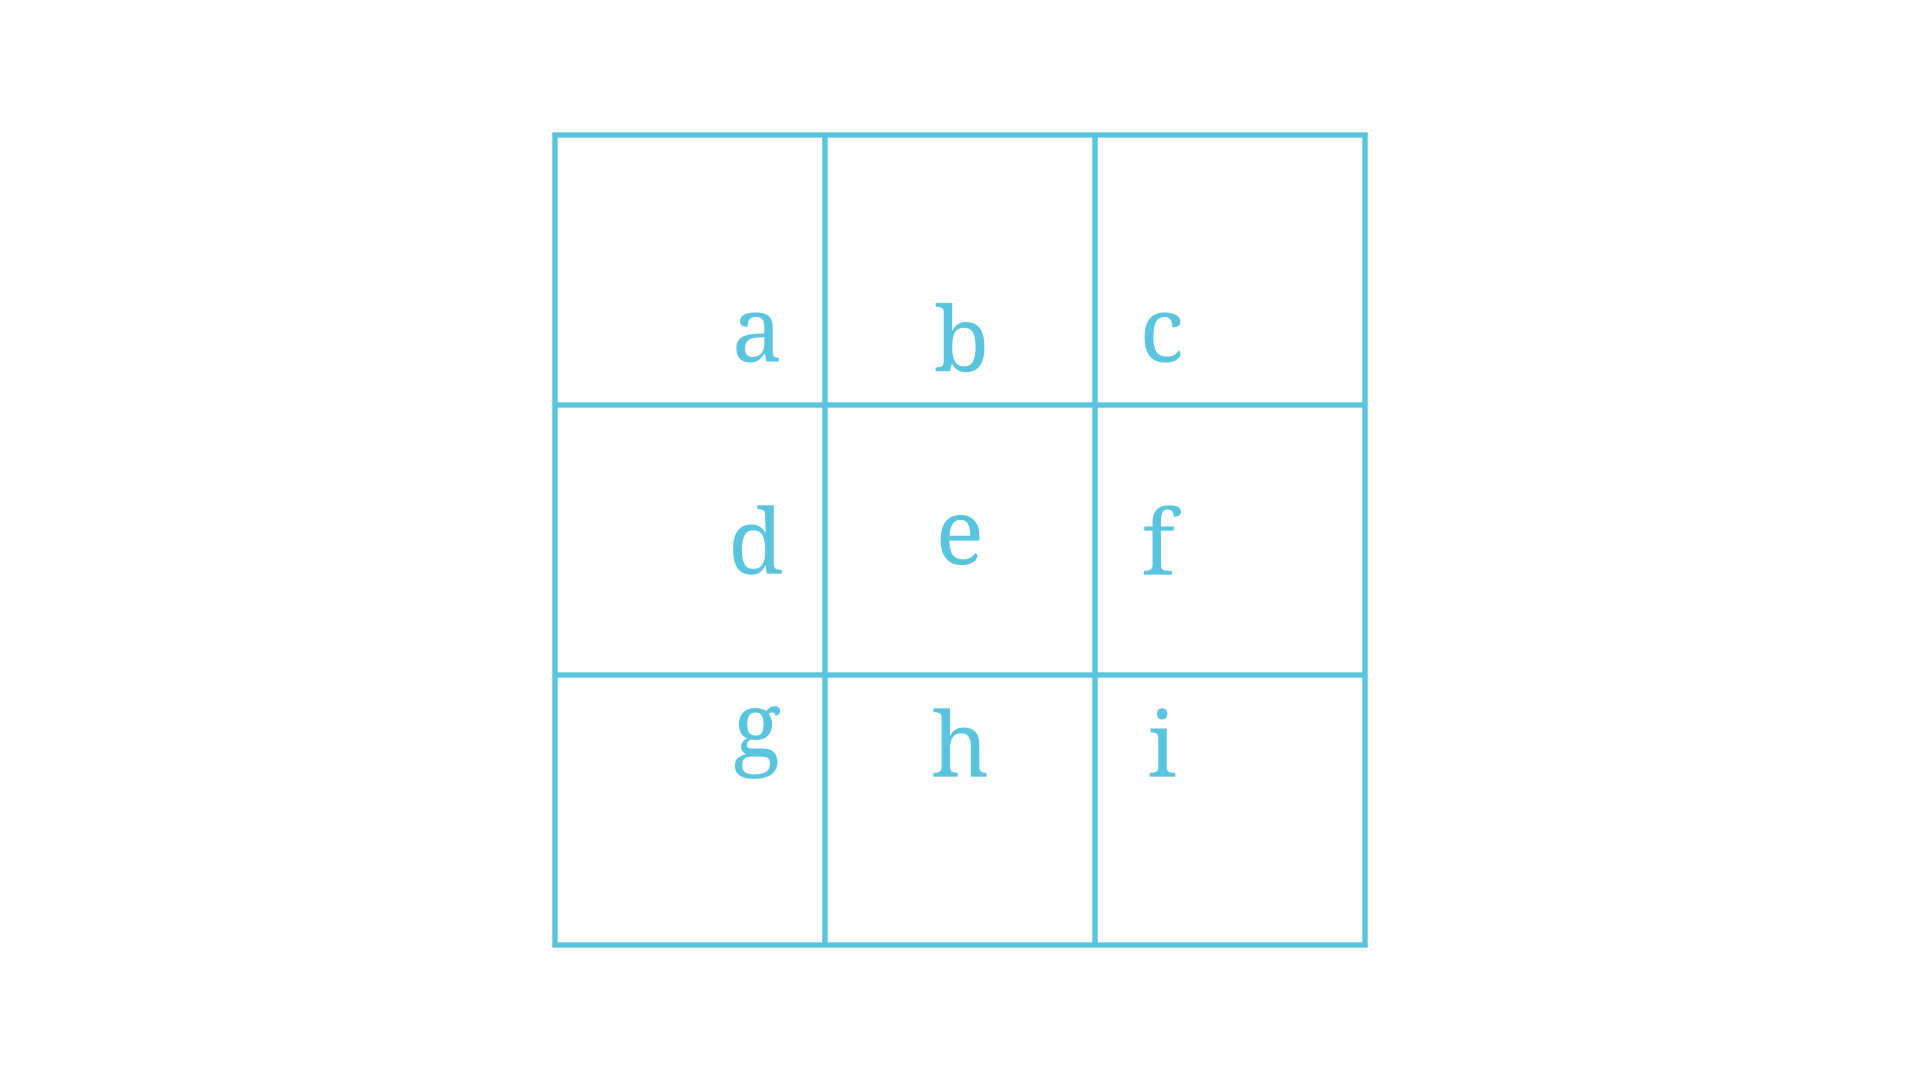
\includegraphics[width=.5\textwidth]{brick-voxel-naming.png}
    \caption{Una posible forma de referirse a cada vóxel de un brick}
    \label{fig:brick-voxel-naming}
\end{figure}

Dado el vóxel superior izquierdo de la figura \ref{fig:svo_filtering_corners}, se considera solo el brick del hijo superior izquierdo del nodo.
De ese brick, se consideran los vóxeles amarillos en la figura.
El valor final del vóxel del padre se calcula promediando los valores de los vóxeles del hijo, pesados por el porcentaje de solapamiento.
Si nombramos los vóxeles del brick hijo $a, \cdots, i$ y los del brick padre $a', \cdots, i'$, como en la figura \ref{fig:brick-voxel-naming}, entonces el valor del vóxel del padre se calcula como:

$$
a' = a + b * \frac{1}{2} + d * \frac{1}{2} + e * \frac{1}{4}
$$

En el caso tridimensional, hay que agregar un quinto factor multiplicado por $\frac{1}{8}$.

% Esto resulta en un kernel gaussiano. % TODO: Alguna referencia sobre kernels gaussianos? Si no no lo mencionamos

\begin{figure}
    \centering
    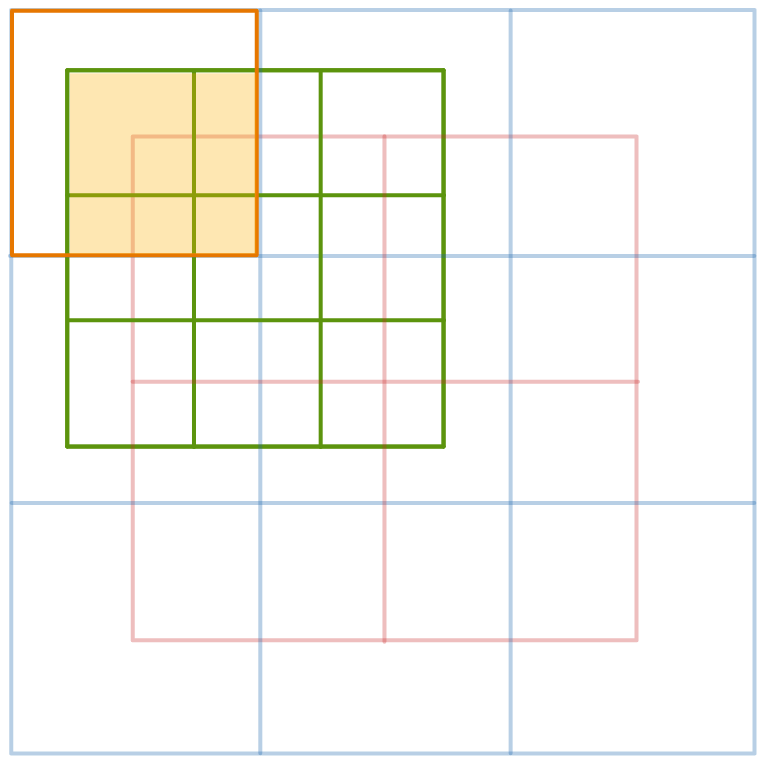
\includegraphics[width=.25\textwidth]{svo-filtering-corner.png}
    \caption{
        Filtrado para un vóxel esquina.
        Se puede ver el vóxel del brick padre cuyo valor se quiere calcular, junto con el brick del hijo y su solapamiento con este vóxel.
    }
    \label{fig:svo_filtering_corners}
\end{figure}

De la misma manera se calculan los vóxels de los bordes y de las caras, solo que en esos casos se usan más de un brick hijo, como se puede ver en las figuras \ref{fig:svo_filtering_edges} y \ref{fig:svo_filtering_faces}.

\begin{figure}
    \begin{center}
        \begin{subfigure}{.24\textwidth}
            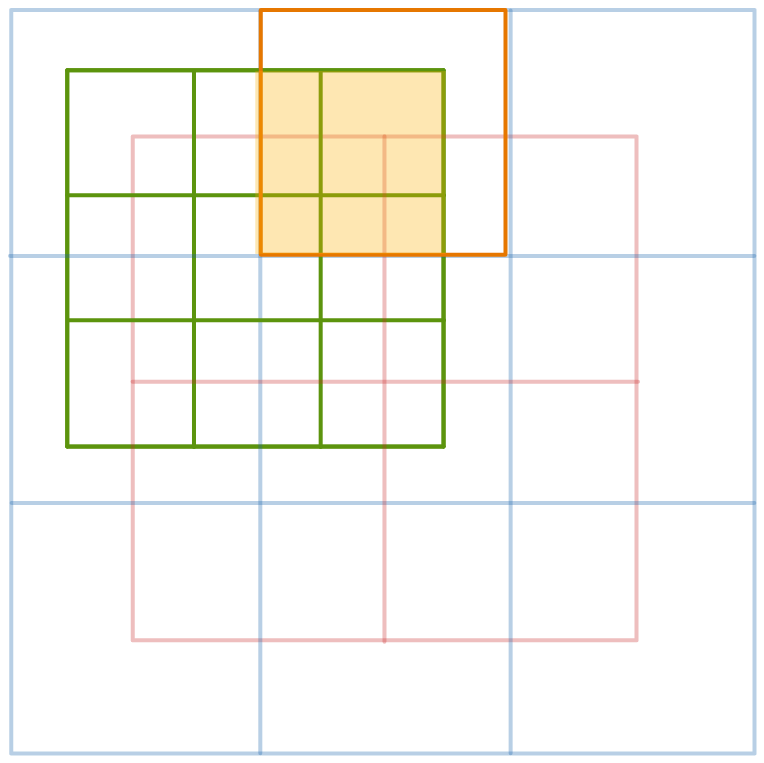
\includegraphics[width=\textwidth]{svo-filtering-edge-1.png}
        \end{subfigure}
        \begin{subfigure}{.24\textwidth}
            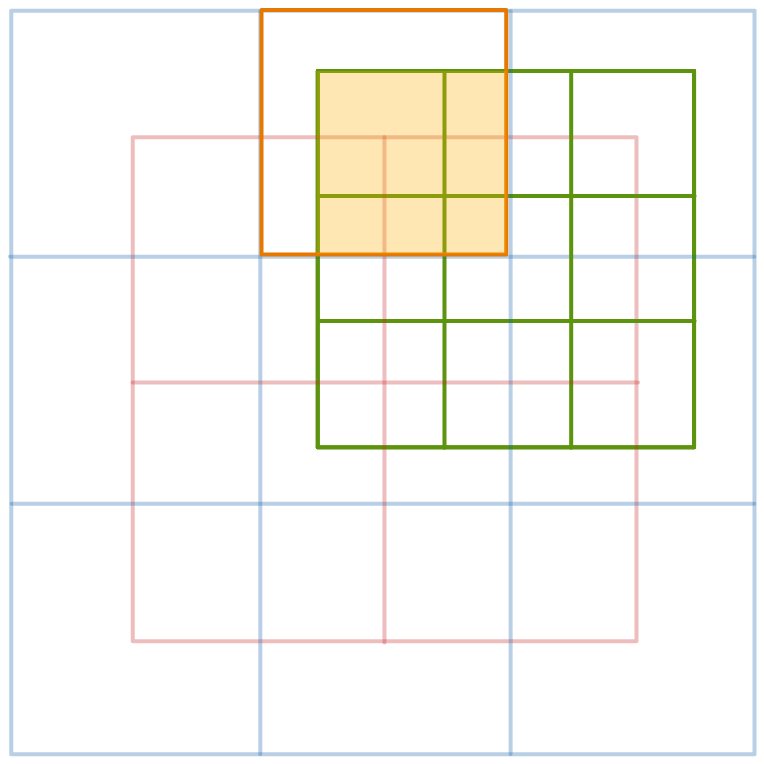
\includegraphics[width=\textwidth]{svo-filtering-edge-2.png}
        \end{subfigure}
    \end{center}
    \caption{Filtrado para un vóxel borde}
    \label{fig:svo_filtering_edges}
\end{figure}

\begin{figure}
    \begin{center}
        \begin{subfigure}{.24\textwidth}
            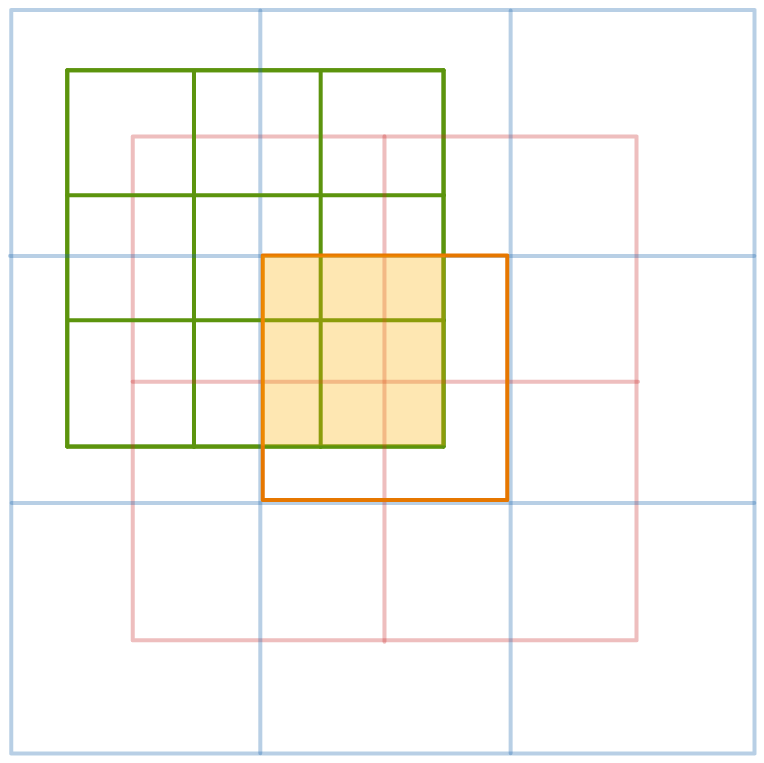
\includegraphics[width=\textwidth]{svo-filtering-face-1.png}
        \end{subfigure}
        \begin{subfigure}{.24\textwidth}
            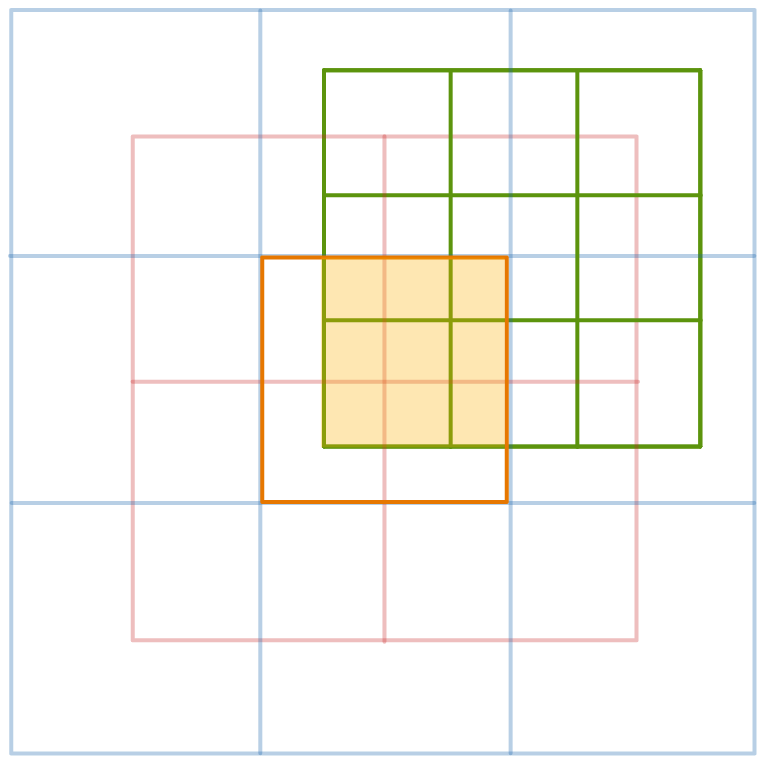
\includegraphics[width=\textwidth]{svo-filtering-face-2.png}
        \end{subfigure}
        \begin{subfigure}{.24\textwidth}
            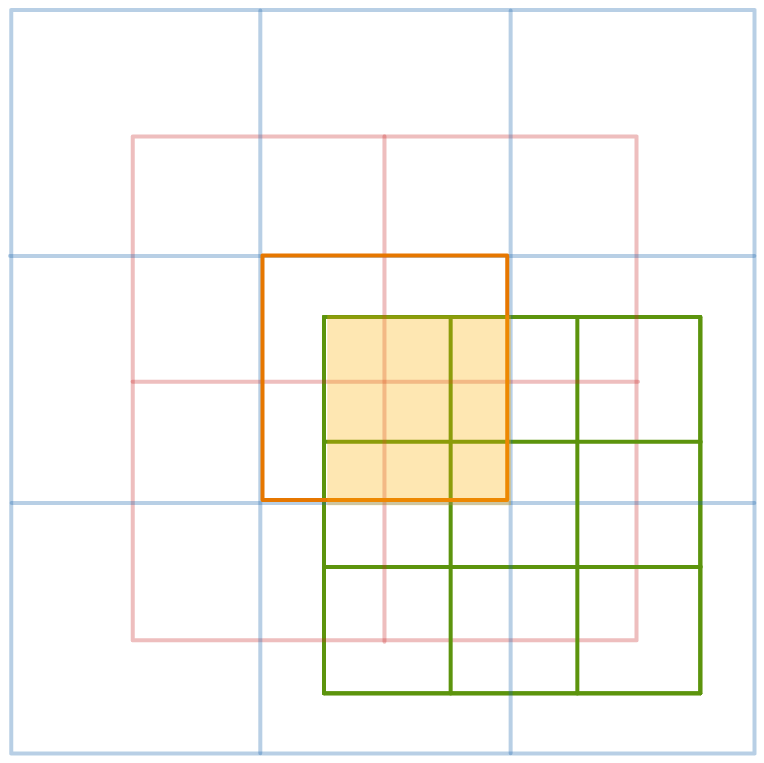
\includegraphics[width=\textwidth]{svo-filtering-face-3.png}
        \end{subfigure}
        \begin{subfigure}{.24\textwidth}
            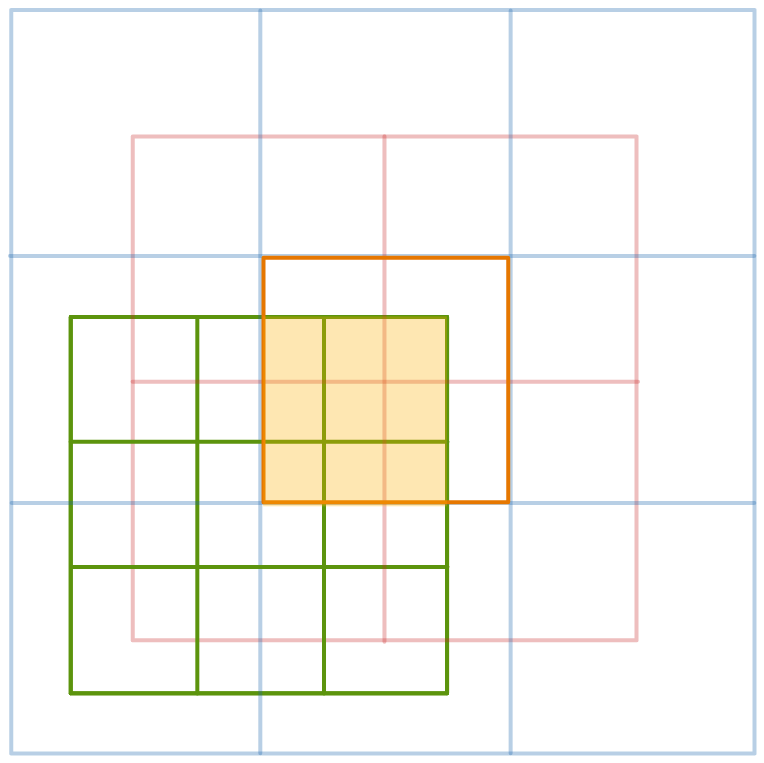
\includegraphics[width=\textwidth]{svo-filtering-face-4.png}
        \end{subfigure}
    \end{center}
    \caption{Filtrado para un vóxel cara}
    \label{fig:svo_filtering_faces}
\end{figure}

% TODO: Solo traer de vuelta si realmente usamos normales en el código.
% Si los vóxels almacenan normales, estas se promedian como se mencionó en la sección \ref{sec:normal_filtering}.

\subsection{Filtrado anisotrópico}

El filtrado descrito en la sección anterior resulta en vóxeles cuyos valores son los mismos vistos en todas las direcciones.
Una propiedad deseable es que se almacenen distintos valores, pudiendo usarse según el ángulo del que se mira.
Esto es muy útil a la hora de representar un atributo como el color en una escena 3D.

Para ver por qué esta propiedad es deseable, consideremos una escena compuesta únicamente por una pared fina.
Dado un vóxel de un nodo alto en el árbol, este representa una gran región del espacio.
Esta región contiene únicamente una pared que pasa por su centro, y el resto es todo espacio vacío.
Con el filtrado presentado anteriormente, llamado \textbf{isotrópico}, este vóxel tendrá un muy bajo valor de opacidad, dado que la mayoría de su espacio es vacío.
Sin embargo, es fácil ver que es muy distinto ver la pared de frente que de costado.
Como se muestra en la figura \ref{fig:anisotropic-thin-wall}, la pared vista de frente es opaca pero vista de costado es mayoritariamente transparente la región que ocupa.

La solución es realizar el filtrado 6 veces por vóxel, uno por cada dirección alineada con los ejes: X, -X, Y, -Y, Z, -Z; y tener en cuenta la dirección a la hora de promediar los valores.
Una vez conseguidos los 6 valores, es posible conseguir cualquier dirección de vista interpolando las tres direcciones más cercanas.
Este filtrado es \textbf{anisotrópico}, no es igual para todas las direcciones.

\begin{figure}
    \centering
    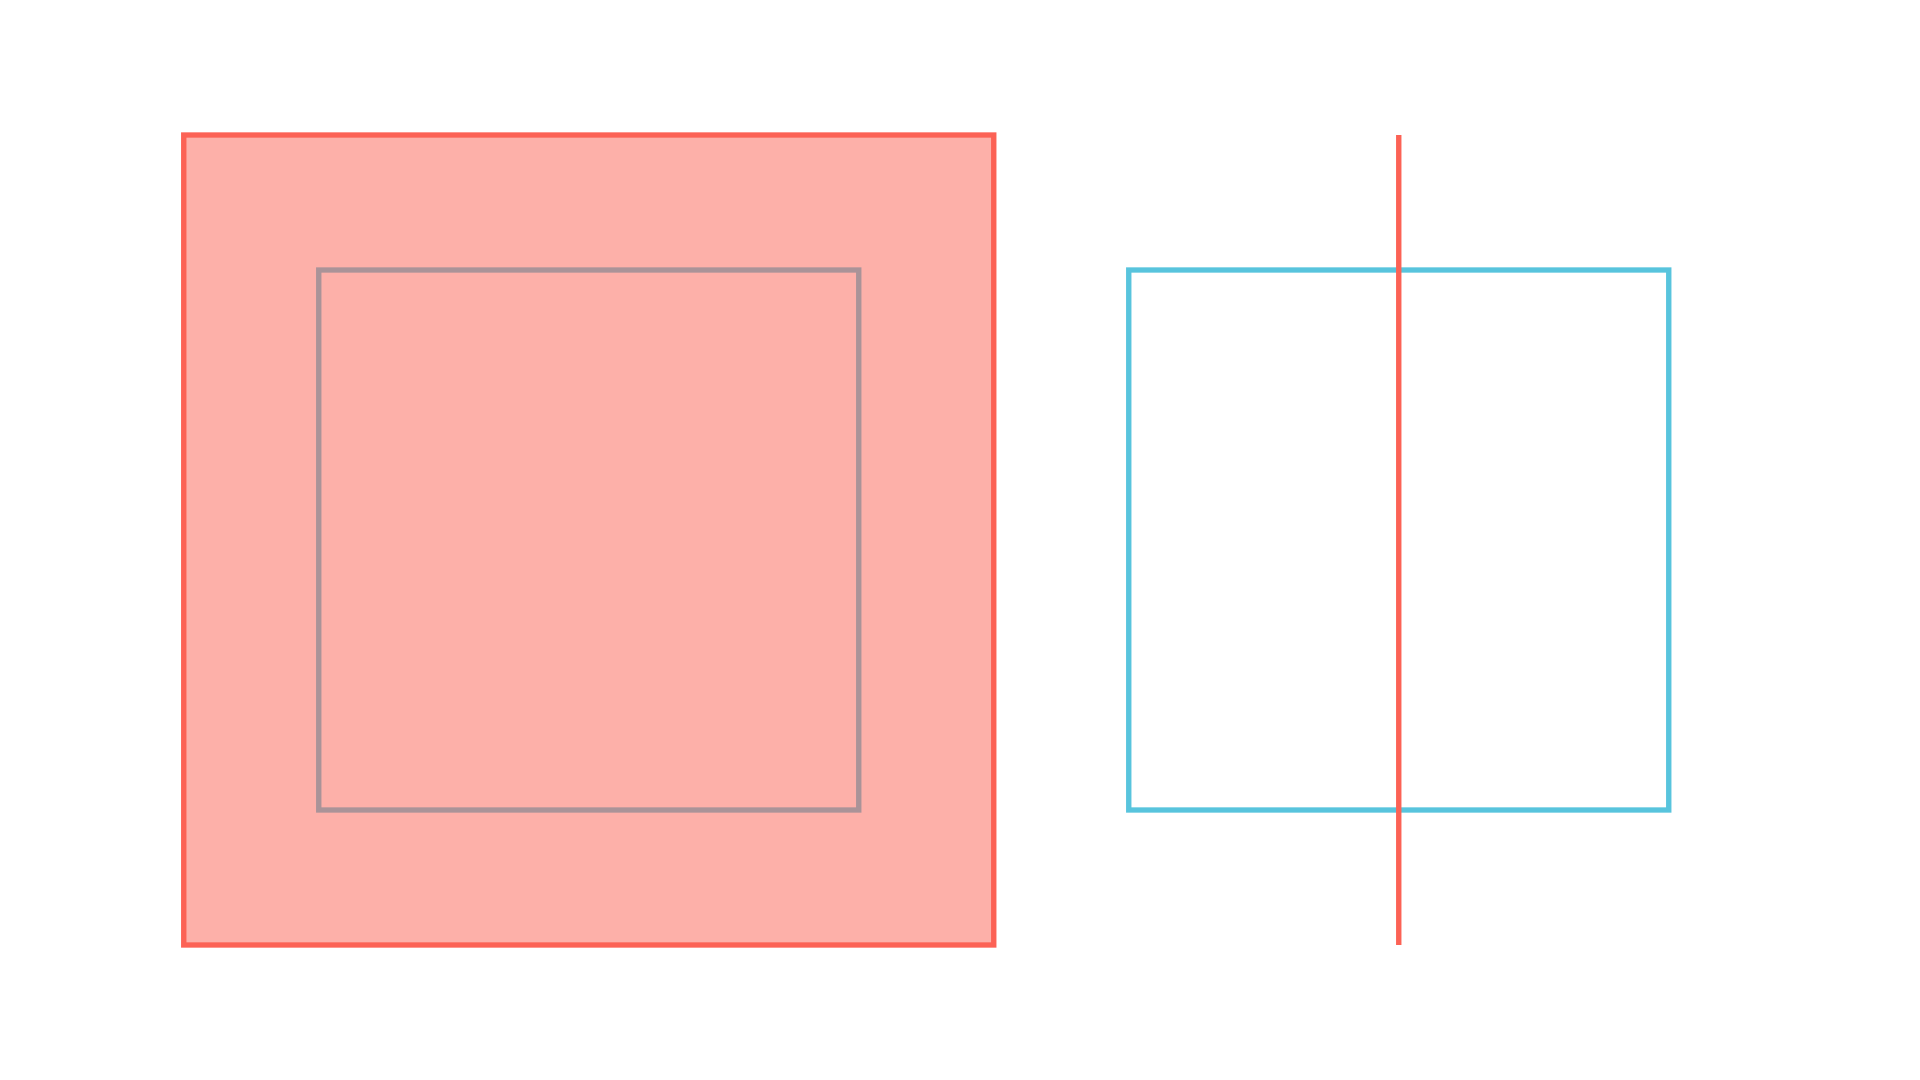
\includegraphics[width=.5\textwidth]{anisotropic-thin-wall.png}
    \caption{
        Vóxel que contiene una pared fina.
        En la izquierda, la pared se ve de frente.
        En la derecha, se ve de costado.
        Se espera que el valor del vóxel refleje esta diferencia entre las direcciones de vista.
    }
    \label{fig:anisotropic-thin-wall}
\end{figure}

Dada una dirección, por ejemplo, de izquierda a derecha, se parte de los vóxeles de la izquierda y se calcula un valor para cada fila, partiendo de estos y yendo hacia los vóxeles de la derecha.
Llamémosle al valor de cada fila \textbf{valor direccional}.
En la figura \ref{fig:svo_filtering_anisotropic} se pueden ver todos los valores direccionales que deben ser calculados para un brick en 2D, para todas las direcciones.
Para cada fila, se ejecuta un algoritmo de acumulación de opacidad que va avanzando en la dirección dada.
Si el algoritmo llega a opacidad 1, termina y devuelve el valor direccional para esa fila.

\begin{figure}
    \begin{center}
        \begin{subfigure}{.24\textwidth}
            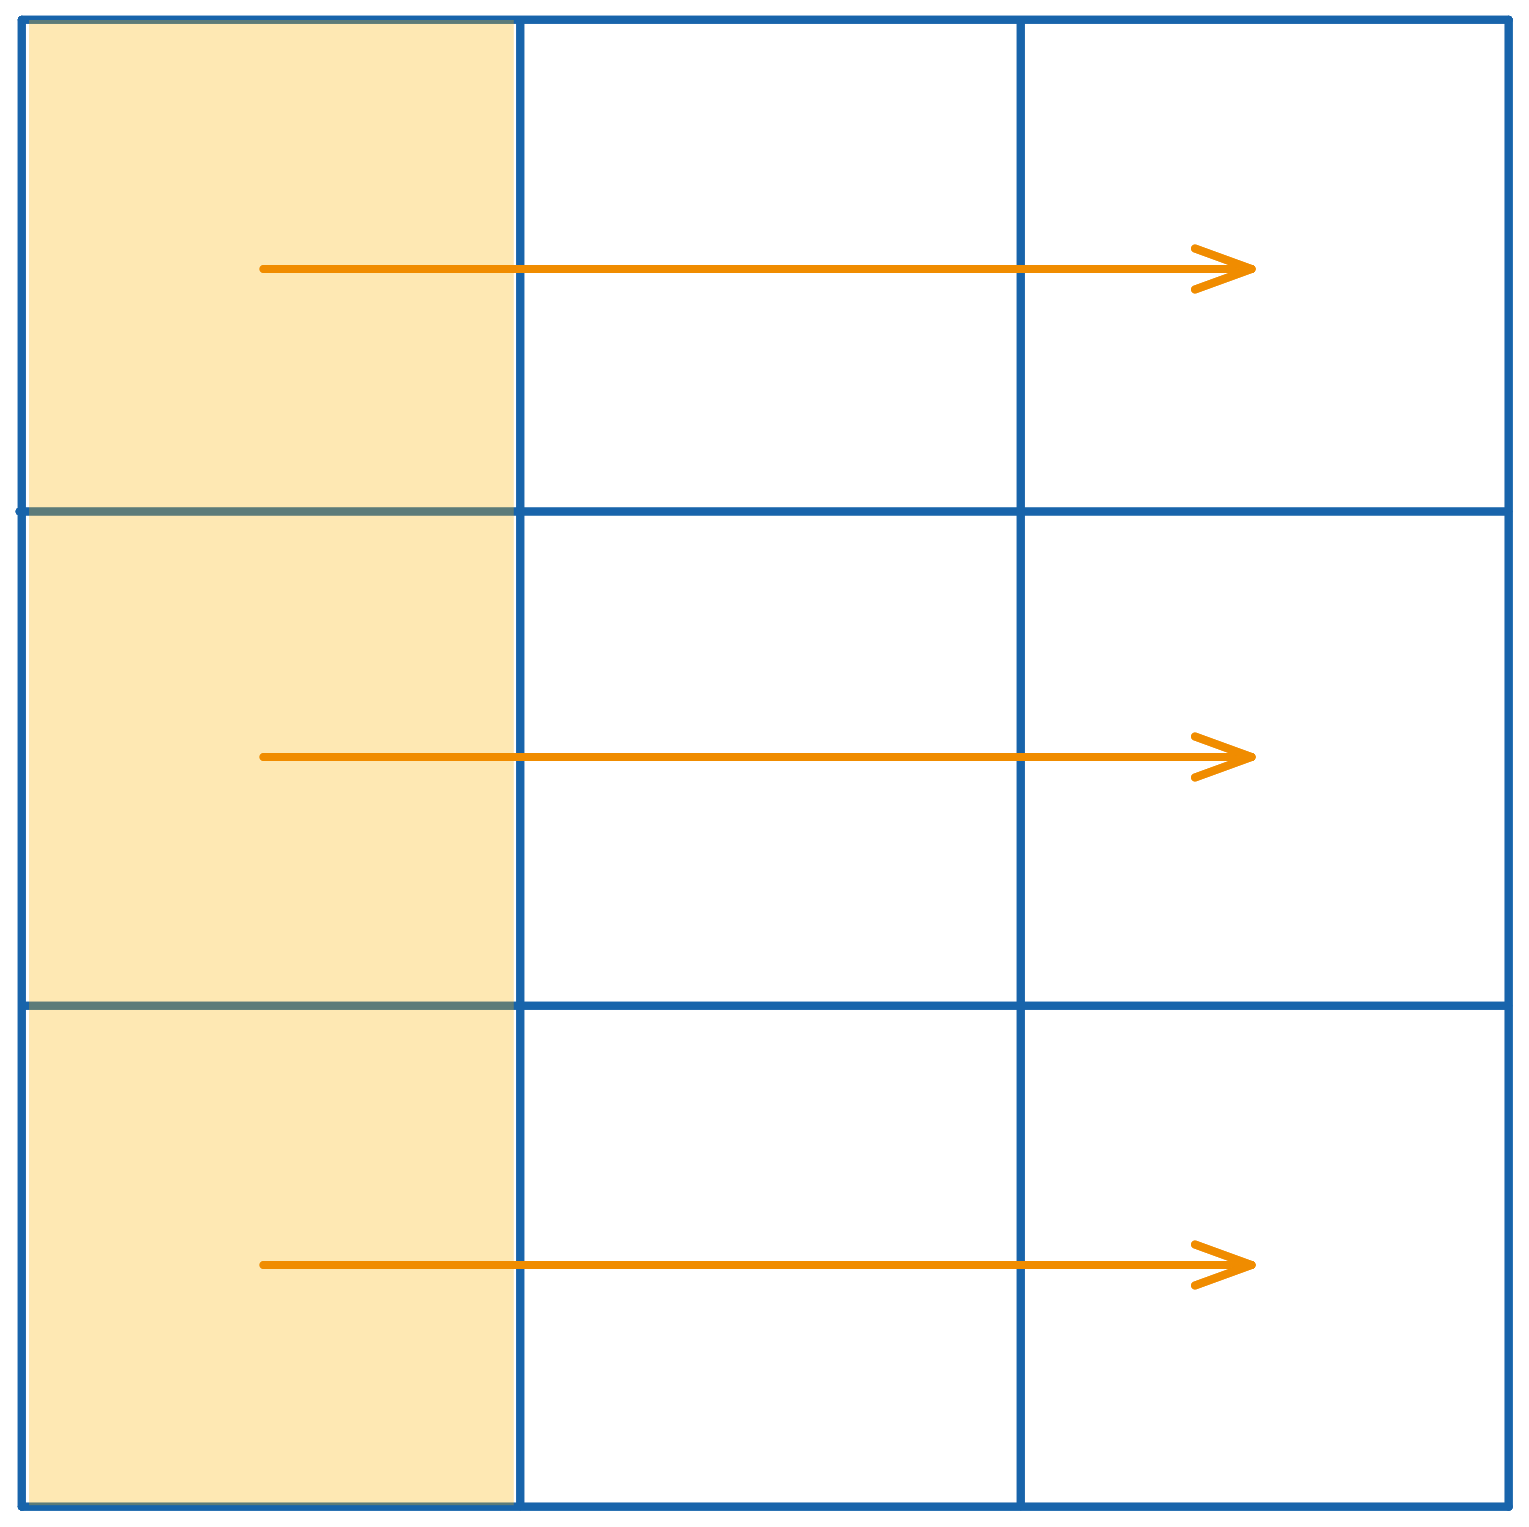
\includegraphics[width=\textwidth]{anisotropic-filtering-x.png}
        \end{subfigure}
        \begin{subfigure}{.24\textwidth}
            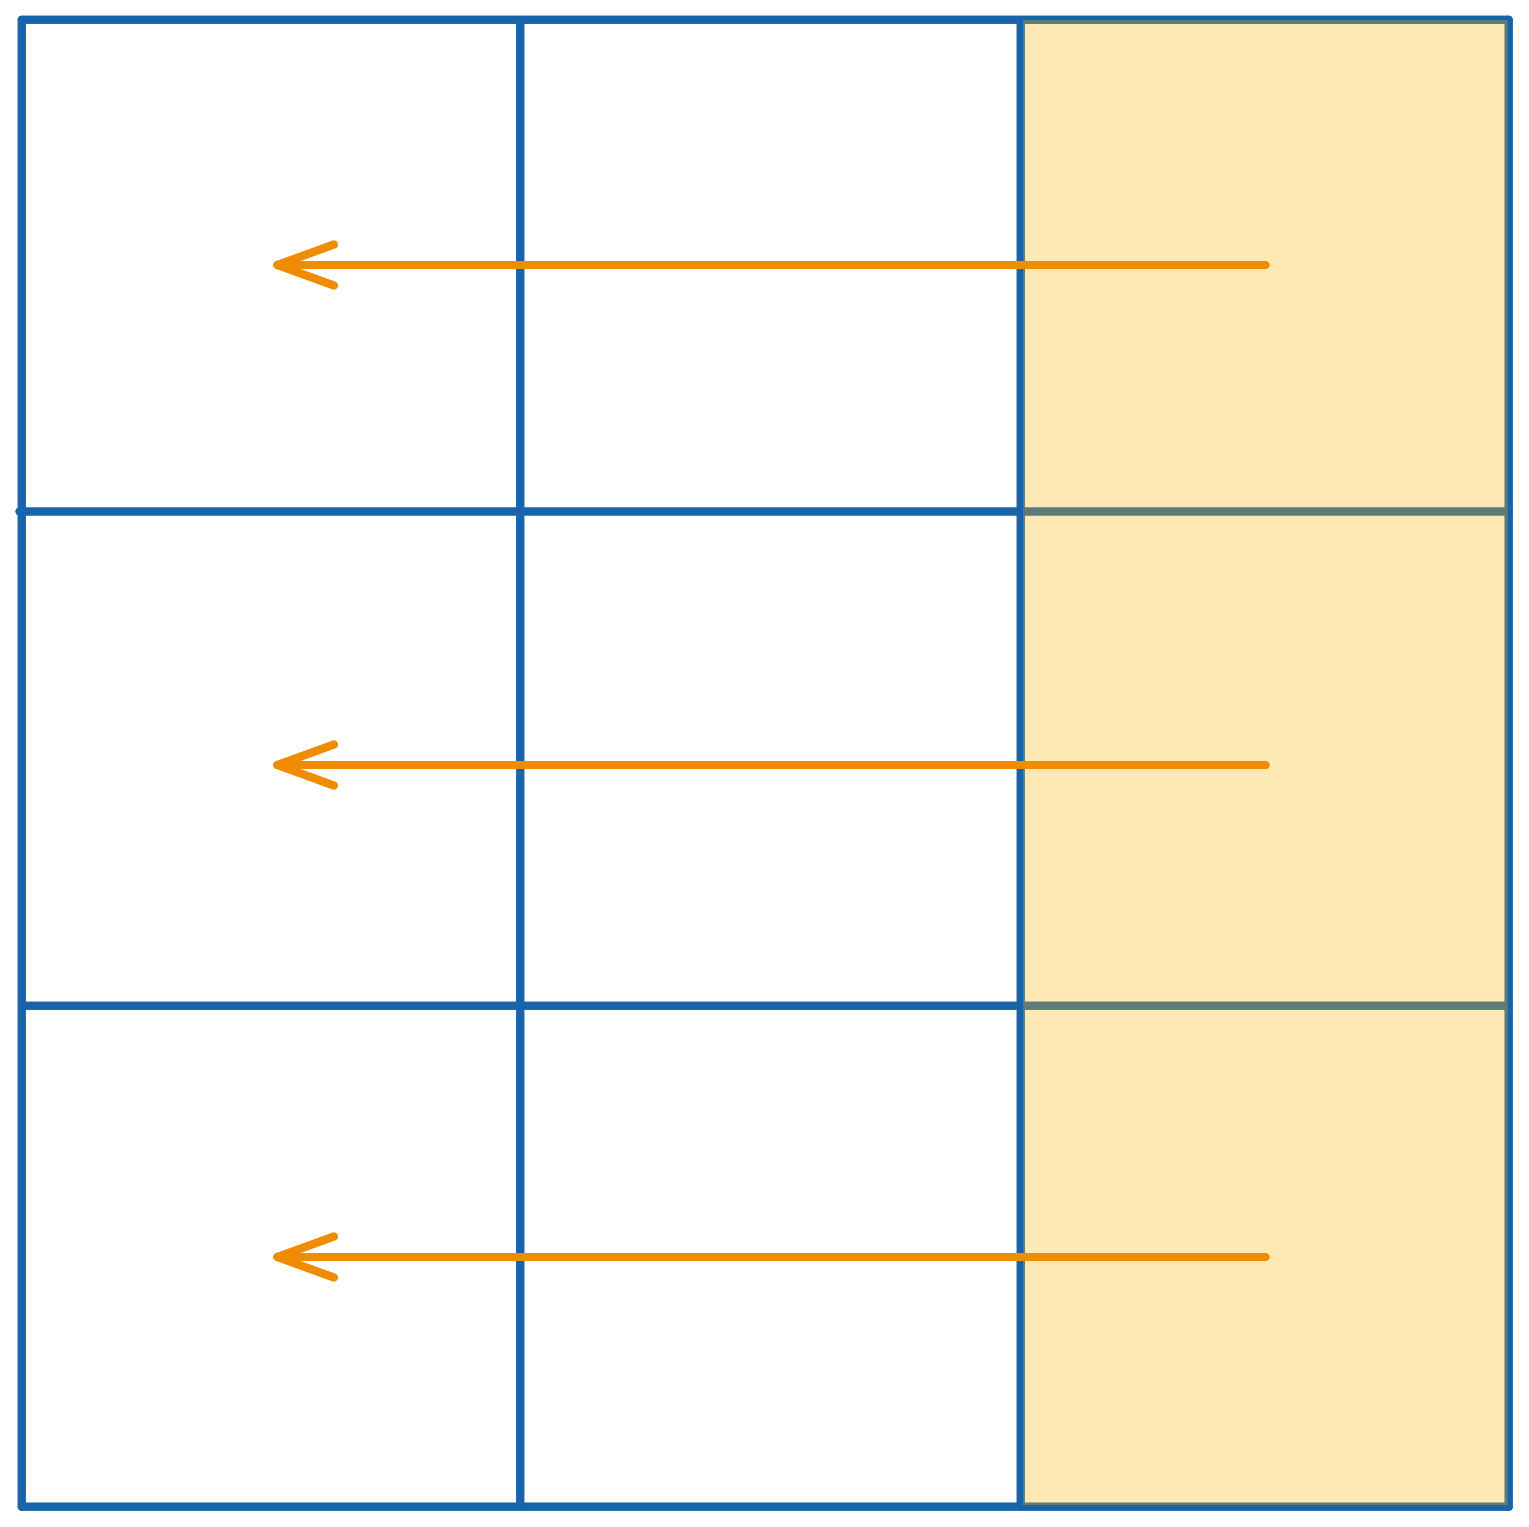
\includegraphics[width=\textwidth]{anisotropic-filtering-x-neg.png}
        \end{subfigure}
        \begin{subfigure}{.24\textwidth}
            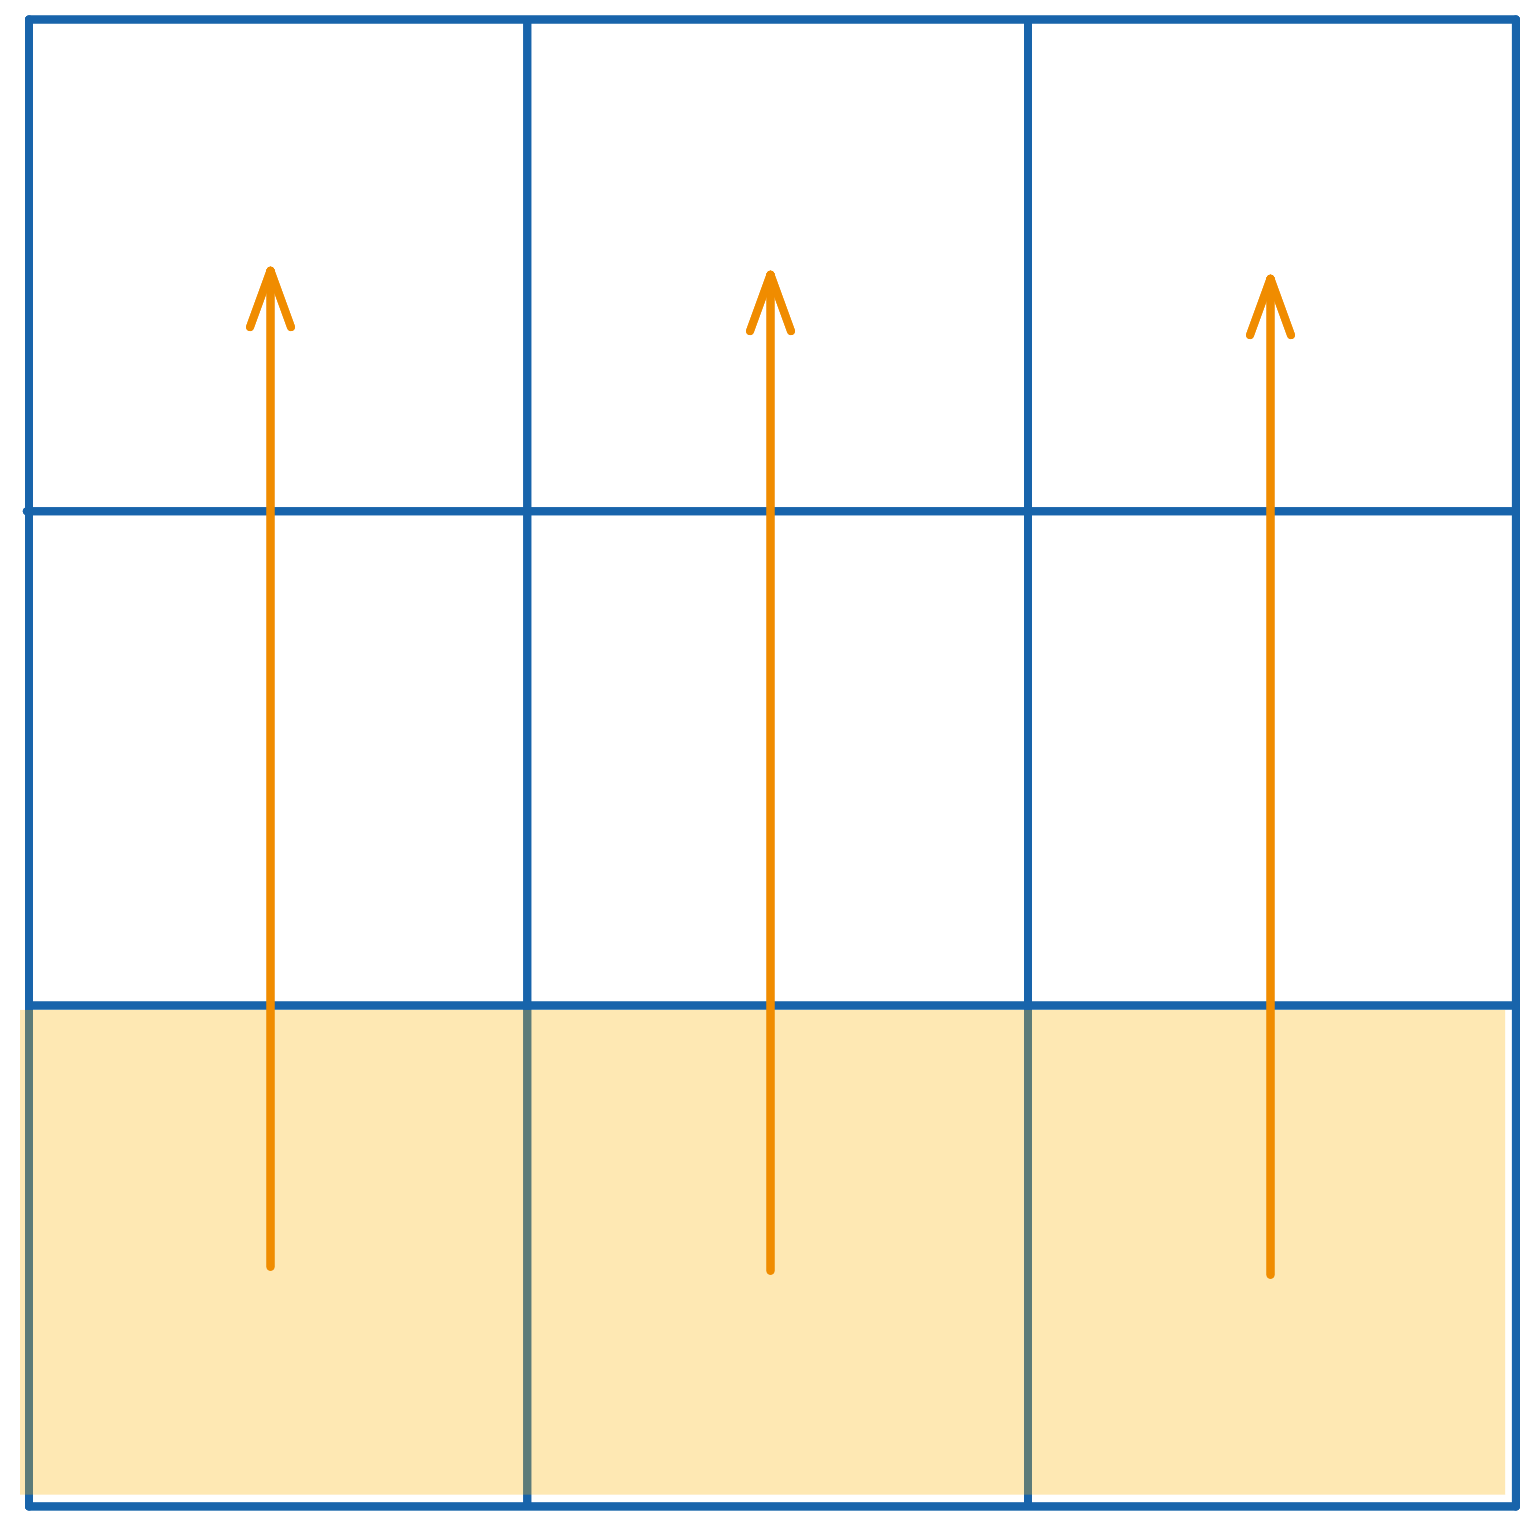
\includegraphics[width=\textwidth]{anisotropic-filtering-y.png}
        \end{subfigure}
        \begin{subfigure}{.24\textwidth}
            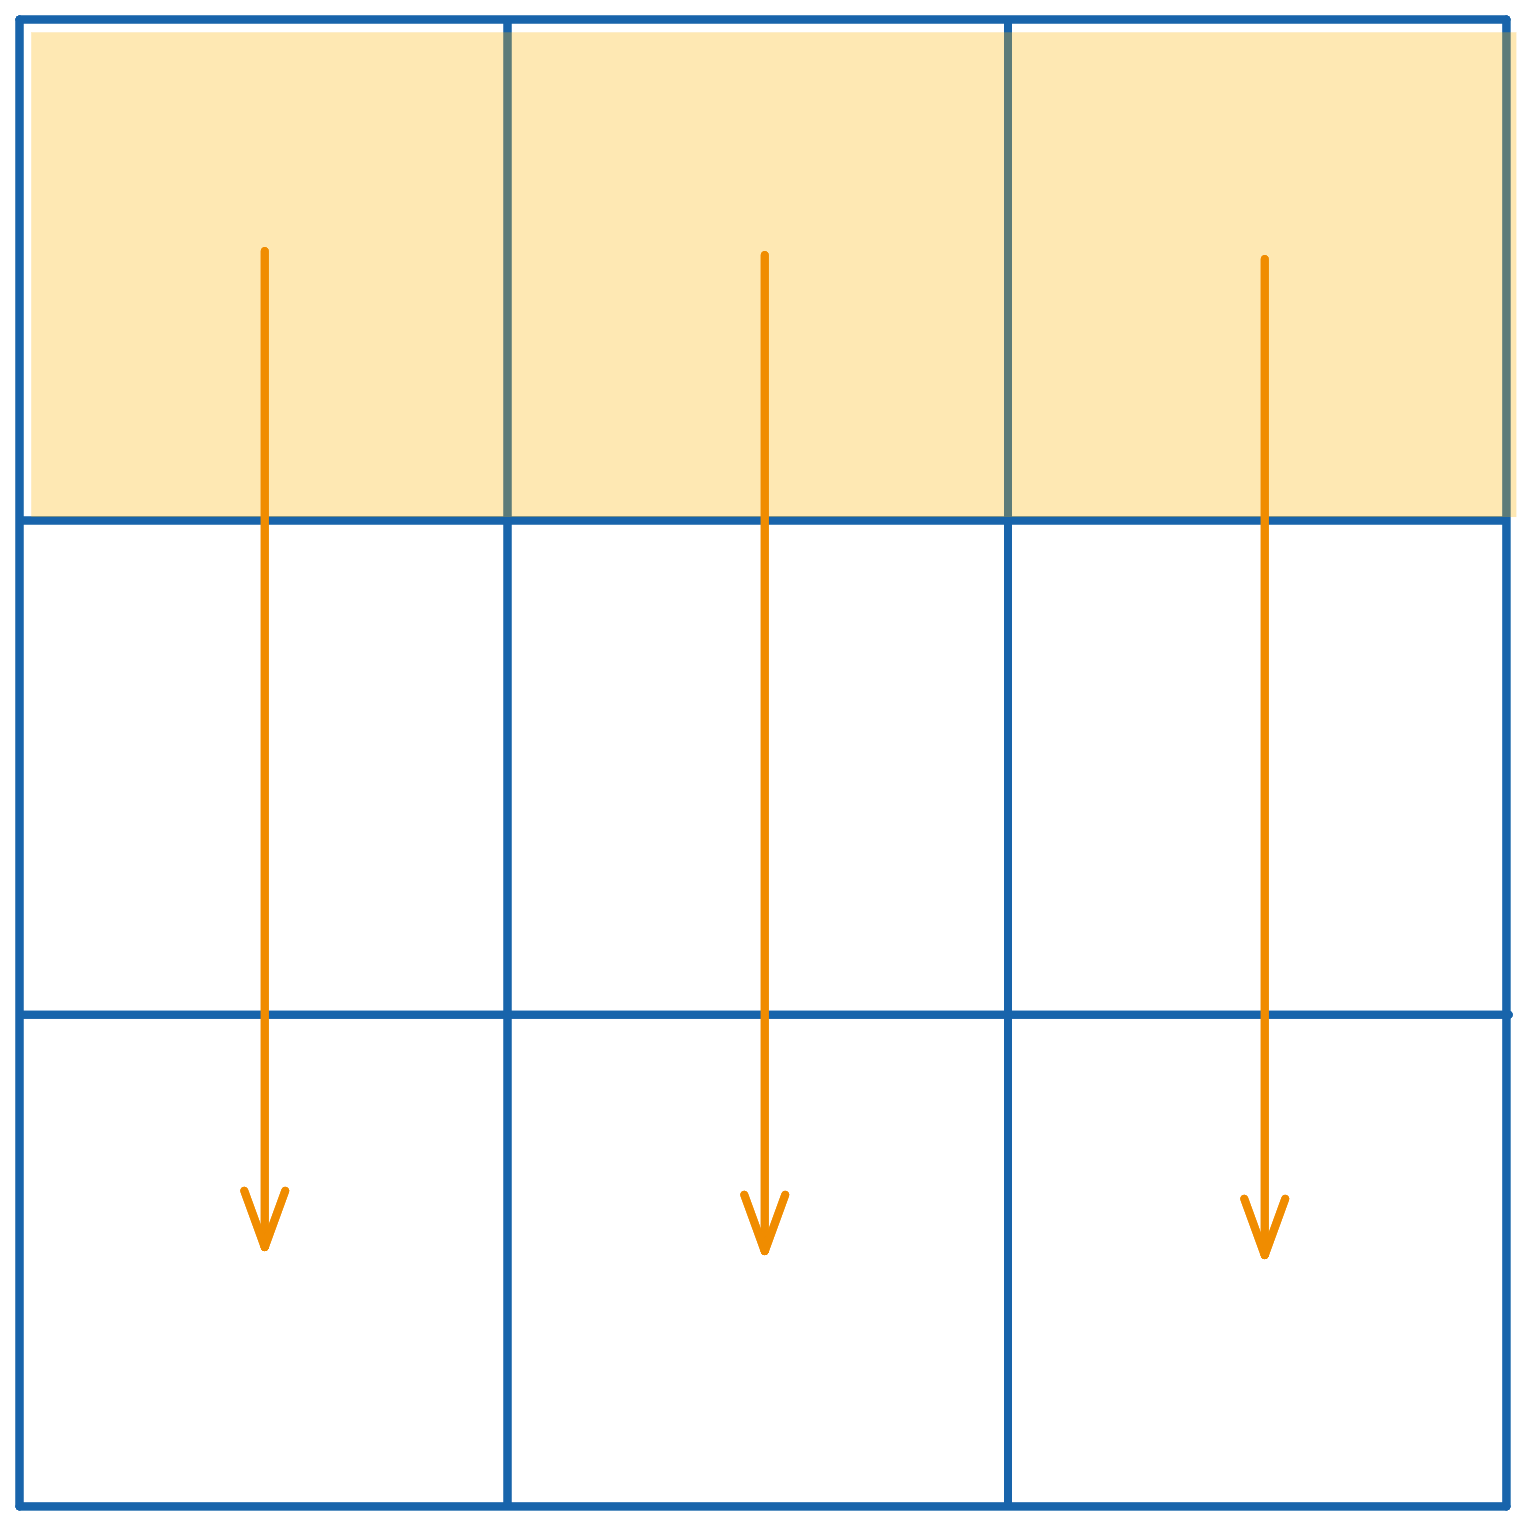
\includegraphics[width=\textwidth]{anisotropic-filtering-y-neg.png}
        \end{subfigure}
    \end{center}
    \caption{Filtrado anisotrópico en todas las direcciones}
    \label{fig:svo_filtering_anisotropic}
\end{figure}

Este tipo de filtrado soluciona situaciones como la de la pared mencionada anteriormente.
Con él, el vóxel que contiene la pared es opaco en la dirección paralela a su normal y transparente en la dirección perpendicular.

\section{Inyección de fotones}\label{sec:photon-injection}

Hasta ahora tenemos la estructura de datos creada, conteniendo el color de toda la escena en las hojas y un promedio de los niveles inferiores en todos los nodos interiores.
El objetivo del algoritmo es la iluminación global de una escena, por lo que necesitamos información de la luz.
En este paso, lanzamos fotones a partir de la fuente de luz de la escena, similar a como se hace en \textit{photon mapping}.
Para hacer esto, se usa el ducto raster.

Se rasteriza la escena del punto de vista de la luz usando el ducto raster para generar una textura 2D.
En lugar de tener colores en cada téxel de esta textura, se almacenan las posiciones de los objetos de la escena.
La existencia de una posición en esta textura significa que esa posición es visible desde la luz, por lo cual debe recibir un fotón.
Las posiciones son utilizadas para recorrer el árbol y almacenar los fotones en vóxeles del mismo.

Los fotones se almacenan en los vóxeles del árbol, esto es la \textbf{irradiancia}, el flujo recibido por la superficie.
Luego pasan por el mismo proceso de \textit{border\_transfer} y filtrado que el color.
El \textit{border\_transfer} suma en lugar de promediar en este caso, dado que ambos lados de la frontera aportan a la cantidad de fotones total.
El filtrado funciona de la misma manera.

La etapa de construcción debe realizarse solo una vez, mientras que, al soportar luces dinámicas, esta etapa debe ejecutarse cada vez que la luz se mueva.
En esos casos, toda la irradiancia del árbol vuelve a cero y se vuelve a correr el programa que lanza los fotones.
A esto se le llama la actualización de la estructura.

% TODO: Quedó extremadamente corta esta parte
% Estaría bueno hablar de las optimizaciones? Te hacen perder un poco

\section{\textit{Cone tracing}}\label{sec:cone_tracing}

Como se comentó brevemente al inicio del capítulo, el trazado de conos se realiza en el \textit{fragment shader} del ducto raster.
La entrada al algoritmo de \textit{cone tracing} son los \textit{geometry buffers} que contienen los valores de la escena, ya habiendo descartado los vértices fuera de vista.
El algoritmo de trazado de conos es ejecutado para cada píxel de los geometry buffers para calcular el color final.

Dado un punto de origen, se lanza uno o varios conos con cierta dirección y apertura, dependiendo del efecto que se quiere lograr.
% TODO: Tema de las normales todo considerando el hemisferio hacia el lado de la normal del punto.

Dado un cono, se parte desde su origen y se avanza en su dirección con un cierto tamaño de paso.
Esto se conoce como \textit{ray marching}. % TODO: No se si está bueno poner el nombre sin haberlo mencionado antes
Después de cada paso tomado, se calcula el diámetro del cono en ese punto.
Dado el diámetro, se calcula un nivel del octree, y dado ese nivel y la posición a lo largo del cono, se recorre el octree y se encuentra el nodo que corresponde a ese nivel y a esa posición.
Ese nodo tiene un brick asociado, cuyos vóxeles tienen los valores prefiltrados, conseguidos en \ref{design:filtering}.
Se usa el valor del vóxel que corresponde con la posición y se acumula.
Se sigue avanzando paso a paso en el cono acumulando valores hasta satisfacer un criterio de parada.
El algoritmo de \textit{cone tracing} en si es simple dado todos los pasos anteriores.

Cada cono calcula un color $c$ y una opacidad $\alpha$.
Si en cada paso consideramos $c$ y $\alpha$ como los valores hasta el momento, y $c_2$ y $\alpha_2$ como los valores nuevos encontrados en el vóxel del paso, entonces en cada paso los valores de $c$ y $\alpha$ se calculan de la siguiente manera:

$$
\begin{cases}
    c = \alpha c + (1 - \alpha) \alpha_2 c_2 \\
    \alpha = \alpha + (1 - \alpha) \alpha_2
\end{cases}
$$

Para la luz indirecta difusa, se lanzan conos para cubrir el hemisferio centrado en la normal del punto.
En la mayoría de los casos, 5 conos anchos difusos dan un buen resultado.
Cada cono acumula el color de los vóxeles con los que se encuentra multiplicado por la cantidad de fotones.
Esto logra un efecto de \textit{light bleed}, donde las superficies adquieren color de otras superficies cercanas que reciben y dispersan luz.

Para la luz indirecta especular, se lanza un solo cono fino en la dirección de reflexión.
Este cono, al ser más fino, se encuentra con nodos de niveles más bajos, con lo que el reflejo tiene mejor definición.
Si se utiliza un mayor ángulo de apertura del cono, el reflejo se ve más turbio, simulando una superficie menos pulida.

\section{Oclusión ambiental}

La oclusión ambiental es una técnica de rendering que se usa para calcular qué tan expuesto está cada punto de una escena a la luz ambiental.
\textit{Cone tracing} se puede usar para calcular este valor.
Este efecto no aporta más al realismo de una escena una vez que se usan los de iluminación indirecta, pero es un buen paso previo para ver el funcionamiento del algoritmo.

Para calcularlo, se lanzan varios conos, cubriendo el hemisferio centrado en la normal del punto.
El único valor necesario es la opacidad.
A medida que se va viajando a lo largo de un cono, se va acumulando la opacidad de los vóxels que se tocan.
Se define una distancia máxima y el criterio de parada es cuando el punto a lo largo del cono pasa esa distancia máxima.

\section{Conos de sombra}

De la misma manera que el trazado de rayos logra sombras lanzando un rayo hacia la fuente de luz, en este caso se logran lanzando un cono hacia la fuente de luz.
El cono toma en cuenta únicamente la opacidad y su criterio de parada es alcanzar la luz o 1 de opacidad antes.
El beneficio de que sea un cono en lugar de un rayo es que se logran sombras suaves, sin necesidad de tener que tomar muchas muestras y promediarlas.

% END.
